\documentclass[aspectratio=169]{beamer}

% Minimal theme
\usetheme{default}
\usecolortheme{dove}

% Remove navigation symbols
\setbeamertemplate{navigation symbols}{}
\setbeamertemplate{footline}{%
  \hfill{\large\insertframenumber\,/\,\inserttotalframenumber}\hspace{0.8em}\vspace{0.5em}%
}

% Colors
\definecolor{popblue}{RGB}{52, 101, 164}
\definecolor{sampred}{RGB}{204, 0, 0}
\definecolor{paramgreen}{RGB}{0, 140, 70}
\definecolor{lightbg}{RGB}{245, 245, 250}
\definecolor{warnred}{RGB}{180, 40, 40}
\definecolor{orange1}{RGB}{220, 120, 0}
\definecolor{violet1}{RGB}{120, 50, 160}

\setbeamercolor{frametitle}{fg=popblue}
\setbeamercolor{title}{fg=popblue}

% Packages
\usepackage{pgfplots}
\usepackage{tikz}
\usetikzlibrary{shapes, arrows.meta, positioning, calc, decorations.pathreplacing, patterns}
\pgfplotsset{compat=1.18}
\usepackage{amsmath, amssymb}
\usepackage{array}
\usepackage{fontenc}

\title{Pre-training \& Fine-tuning}
\subtitle{CLM $\cdot$ MLM $\cdot$ NSP $\cdot$ SFT $\cdot$ RLHF $\cdot$ DPO $\cdot$ LoRA}
\date{}

\begin{document}

% ============================================================
% TITLE
% ============================================================
\begin{frame}
\titlepage
\end{frame}

% ============================================================
% THE TWO-STAGE PARADIGM
% ============================================================
\begin{frame}
\frametitle{The two-stage paradigm}

\begin{center}
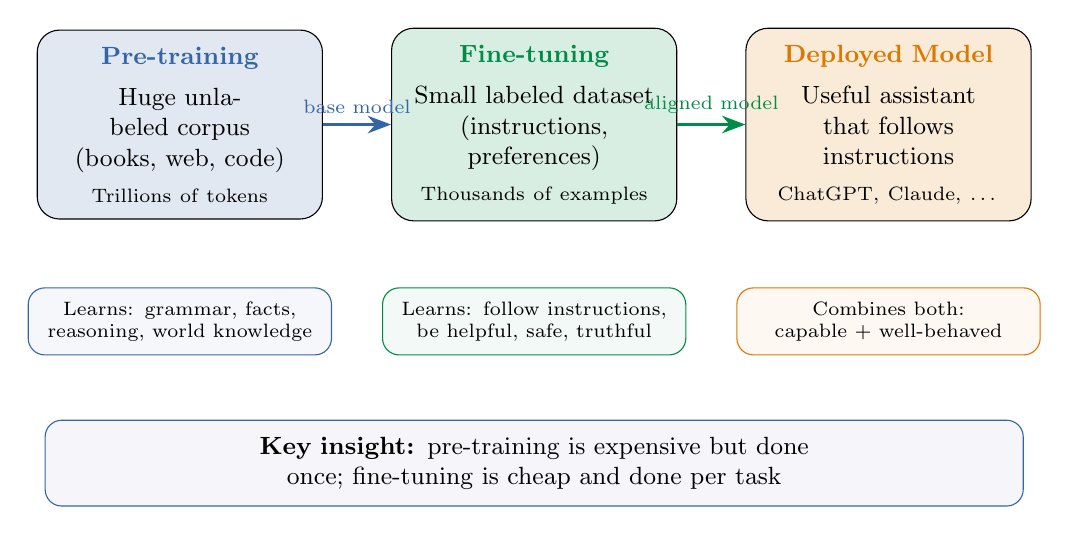
\begin{tikzpicture}
  % Stage 1: Pre-training
  \node[draw, rounded corners=8pt, fill=popblue!15, minimum width=3.5cm, minimum height=2cm, text width=3.2cm, align=center, inner sep=6pt, font=\small] (pt) at (-4.5, 1.5) {
    \textbf{\textcolor{popblue}{Pre-training}}\\[4pt]
    Huge unlabeled corpus\\(books, web, code)\\[2pt]
    {\scriptsize Trillions of tokens}
  };

  % Stage 2: Fine-tuning
  \node[draw, rounded corners=8pt, fill=paramgreen!15, minimum width=3.5cm, minimum height=2cm, text width=3.2cm, align=center, inner sep=6pt, font=\small] (ft) at (0, 1.5) {
    \textbf{\textcolor{paramgreen}{Fine-tuning}}\\[4pt]
    Small labeled dataset\\(instructions, preferences)\\[2pt]
    {\scriptsize Thousands of examples}
  };

  % Deploy
  \node[draw, rounded corners=8pt, fill=orange1!15, minimum width=3.5cm, minimum height=2cm, text width=3.2cm, align=center, inner sep=6pt, font=\small] (dep) at (4.5, 1.5) {
    \textbf{\textcolor{orange1}{Deployed Model}}\\[4pt]
    Useful assistant\\that follows instructions\\[2pt]
    {\scriptsize ChatGPT, Claude, \ldots}
  };

  % Arrows
  \draw[-Stealth, very thick, popblue] (pt) -- (ft) node[midway, above, font=\scriptsize] {base model};
  \draw[-Stealth, very thick, paramgreen] (ft) -- (dep) node[midway, above, font=\scriptsize] {aligned model};

  % What each stage learns
  \node[draw=popblue, fill=popblue!5, rounded corners=6pt, text width=3.5cm, align=center, inner sep=5pt, font=\scriptsize] at (-4.5, -1) {
    Learns: grammar, facts,\\reasoning, world knowledge
  };
  \node[draw=paramgreen, fill=paramgreen!5, rounded corners=6pt, text width=3.5cm, align=center, inner sep=5pt, font=\scriptsize] at (0, -1) {
    Learns: follow instructions,\\be helpful, safe, truthful
  };
  \node[draw=orange1, fill=orange1!5, rounded corners=6pt, text width=3.5cm, align=center, inner sep=5pt, font=\scriptsize] at (4.5, -1) {
    Combines both:\\capable + well-behaved
  };

  % Bottom note
  \node[draw=popblue, fill=lightbg, rounded corners=6pt, text width=12cm, align=center, inner sep=6pt, font=\small] at (0, -2.8) {
    \textbf{Key insight:} pre-training is expensive but done once; fine-tuning is cheap and done per task
  };
\end{tikzpicture}
\end{center}
\end{frame}

% ============================================================
% PART I HEADER
% ============================================================
\begin{frame}
\begin{center}
\vspace{1.5cm}
{\Huge \textcolor{popblue}{Part I}}

\vspace{0.5cm}
{\Large Pre-training Objectives}

\vspace{0.5cm}
{\normalsize How models learn from raw text}
\end{center}
\end{frame}

% ============================================================
% CAUSAL LANGUAGE MODELING
% ============================================================
\begin{frame}
\frametitle{Causal Language Modeling (CLM)}

\vspace{-0.2cm}
\begin{center}
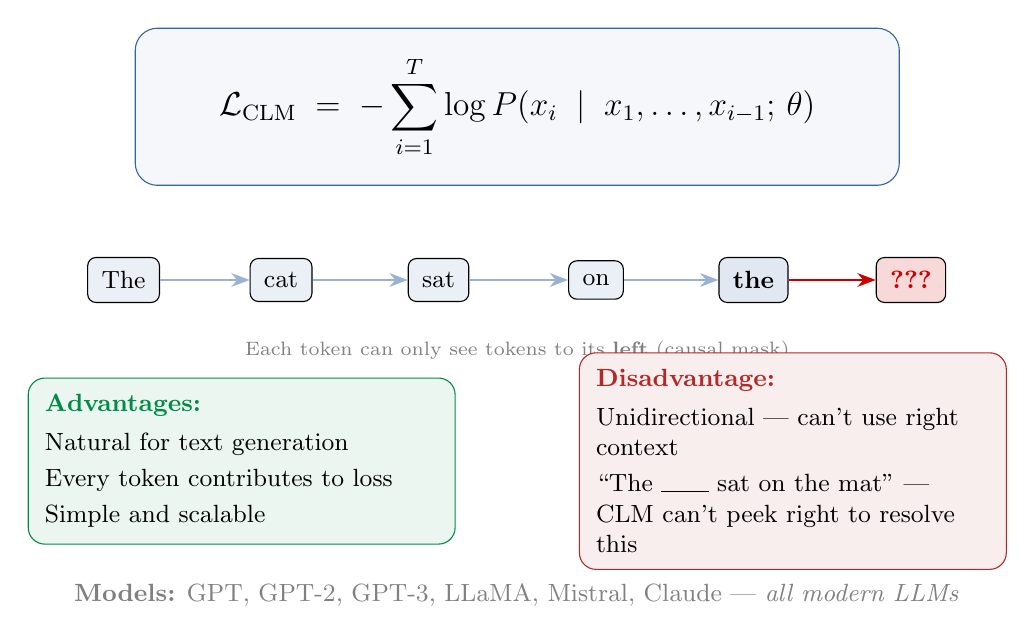
\begin{tikzpicture}
  % Formula
  \node[draw=popblue, fill=popblue!5, rounded corners=8pt, inner sep=10pt, text width=9cm, align=center] at (0, 3) {
    {\large $\displaystyle \mathcal{L}_{\text{CLM}} = -\sum_{i=1}^{T} \log P(x_i \mid x_1, \ldots, x_{i-1};\, \theta)$}
  };

  % Causal sequence
  \node[draw, rounded corners=3pt, fill=popblue!10, inner sep=5pt, font=\small] (t1) at (-5, 0.8) {The};
  \node[draw, rounded corners=3pt, fill=popblue!10, inner sep=5pt, font=\small] (t2) at (-3, 0.8) {cat};
  \node[draw, rounded corners=3pt, fill=popblue!10, inner sep=5pt, font=\small] (t3) at (-1, 0.8) {sat};
  \node[draw, rounded corners=3pt, fill=popblue!10, inner sep=5pt, font=\small] (t4) at (1, 0.8) {on};
  \node[draw, rounded corners=3pt, fill=popblue!15, inner sep=5pt, font=\small\bfseries] (t5) at (3, 0.8) {the};
  \node[draw, rounded corners=3pt, fill=sampred!15, inner sep=5pt, font=\small\bfseries, text=sampred] (t6) at (5, 0.8) {???};

  % Arrows showing causal direction
  \draw[-Stealth, thick, popblue!50] (t1) -- (t2);
  \draw[-Stealth, thick, popblue!50] (t2) -- (t3);
  \draw[-Stealth, thick, popblue!50] (t3) -- (t4);
  \draw[-Stealth, thick, popblue!50] (t4) -- (t5);
  \draw[-Stealth, thick, sampred] (t5) -- (t6);

  % Causal mask visualization
  \node[font=\scriptsize, text=gray] at (0, -0.1) {Each token can only see tokens to its \textbf{left} (causal mask)};

  % Pros and cons
  \node[draw=paramgreen, fill=paramgreen!8, rounded corners=6pt, text width=5cm, align=left, inner sep=6pt, font=\small] at (-3.5, -1.5) {
    \textbf{\textcolor{paramgreen}{Advantages:}}\\[3pt]
    Natural for text generation\\[2pt]
    Every token contributes to loss\\[2pt]
    Simple and scalable
  };
  \node[draw=warnred, fill=warnred!8, rounded corners=6pt, text width=5cm, align=left, inner sep=6pt, font=\small] at (3.5, -1.5) {
    \textbf{\textcolor{warnred}{Disadvantage:}}\\[3pt]
    Unidirectional --- can't use right context\\[2pt]
    ``The \rule{0.6cm}{0.4pt} sat on the mat'' --- CLM can't peek right to resolve this
  };

  % Models
  \node[font=\small, text=gray] at (0, -3.2) {
    \textbf{Models:} GPT, GPT-2, GPT-3, LLaMA, Mistral, Claude --- \emph{all modern LLMs}
  };
\end{tikzpicture}
\end{center}
\end{frame}

% ============================================================
% MASKED LANGUAGE MODELING
% ============================================================
\begin{frame}
\frametitle{Masked Language Modeling (MLM)}

\vspace{-0.6cm}
\begin{center}
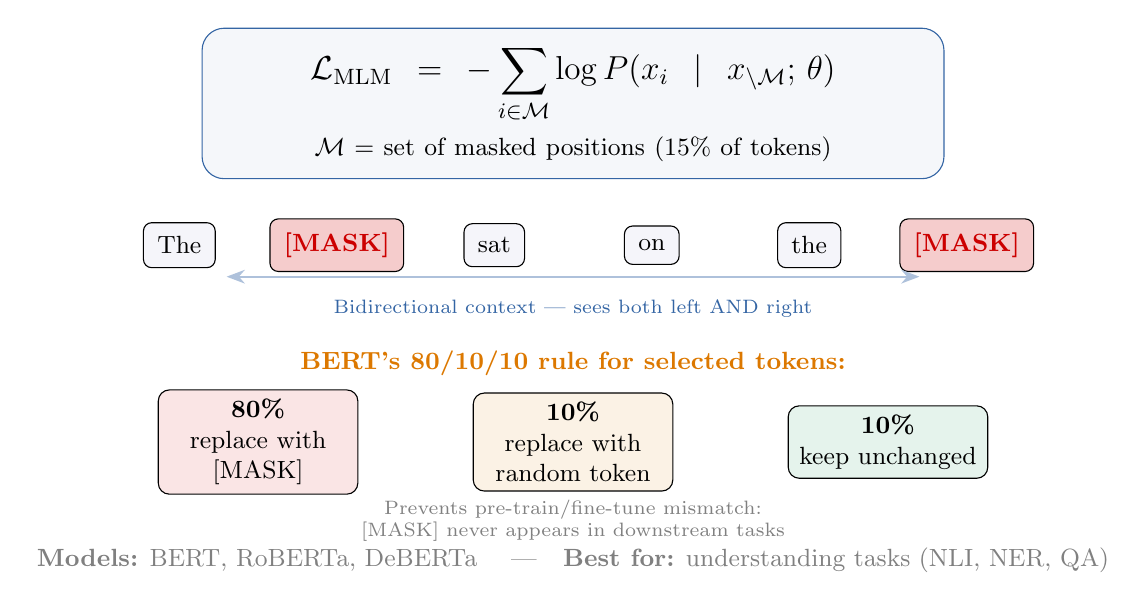
\begin{tikzpicture}
  % Formula
  \node[draw=popblue, fill=popblue!5, rounded corners=8pt, inner sep=6pt, text width=9cm, align=center] at (0, 2.8) {
    {\large $\displaystyle \mathcal{L}_{\text{MLM}} = -\sum_{i \in \mathcal{M}} \log P(x_i \mid x_{\setminus \mathcal{M}};\, \theta)$}\\[4pt]
    {\small $\mathcal{M}$ = set of masked positions (15\% of tokens)}
  };

  % Sentence with masks
  \node[draw, rounded corners=3pt, fill=lightbg, inner sep=5pt, font=\small] at (-5, 1) {The};
  \node[draw, rounded corners=3pt, fill=sampred!20, inner sep=5pt, font=\small\bfseries, text=sampred] at (-3, 1) {[MASK]};
  \node[draw, rounded corners=3pt, fill=lightbg, inner sep=5pt, font=\small] at (-1, 1) {sat};
  \node[draw, rounded corners=3pt, fill=lightbg, inner sep=5pt, font=\small] at (1, 1) {on};
  \node[draw, rounded corners=3pt, fill=lightbg, inner sep=5pt, font=\small] at (3, 1) {the};
  \node[draw, rounded corners=3pt, fill=sampred!20, inner sep=5pt, font=\small\bfseries, text=sampred] at (5, 1) {[MASK]};

  % Bidirectional arrows
  \draw[Stealth-Stealth, thick, popblue!40] (-4.4, 0.6) -- (4.4, 0.6);
  \node[font=\scriptsize, text=popblue] at (0, 0.2) {Bidirectional context --- sees both left AND right};

  % 80/10/10 rule
  \node[font=\small\bfseries, text=orange1] at (0, -0.5) {BERT's 80/10/10 rule for selected tokens:};

  \node[draw, rounded corners=4pt, fill=sampred!10, minimum width=2.5cm, font=\small, text width=2.3cm, align=center] at (-4, -1.5) {
    \textbf{80\%}\\replace with [MASK]
  };
  \node[draw, rounded corners=4pt, fill=orange1!10, minimum width=2.5cm, font=\small, text width=2.3cm, align=center] at (0, -1.5) {
    \textbf{10\%}\\replace with random token
  };
  \node[draw, rounded corners=4pt, fill=paramgreen!10, minimum width=2.5cm, font=\small, text width=2.3cm, align=center] at (4, -1.5) {
    \textbf{10\%}\\keep unchanged
  };

  % Why: prevent mismatch
  \node[font=\scriptsize, text=gray, text width=10cm, align=center] at (0, -2.5) {
    Prevents pre-train/fine-tune mismatch: [MASK] never appears in downstream tasks
  };

  % Models
  \node[font=\small, text=gray] at (0, -3.0) {
    \textbf{Models:} BERT, RoBERTa, DeBERTa \quad |\quad \textbf{Best for:} understanding tasks (NLI, NER, QA)
  };
\end{tikzpicture}
\end{center}
\end{frame}

% ============================================================
% NSP & SOP
% ============================================================
\begin{frame}
\frametitle{Next Sentence Prediction (NSP) \& Sentence Order Prediction (SOP)}

\begin{center}
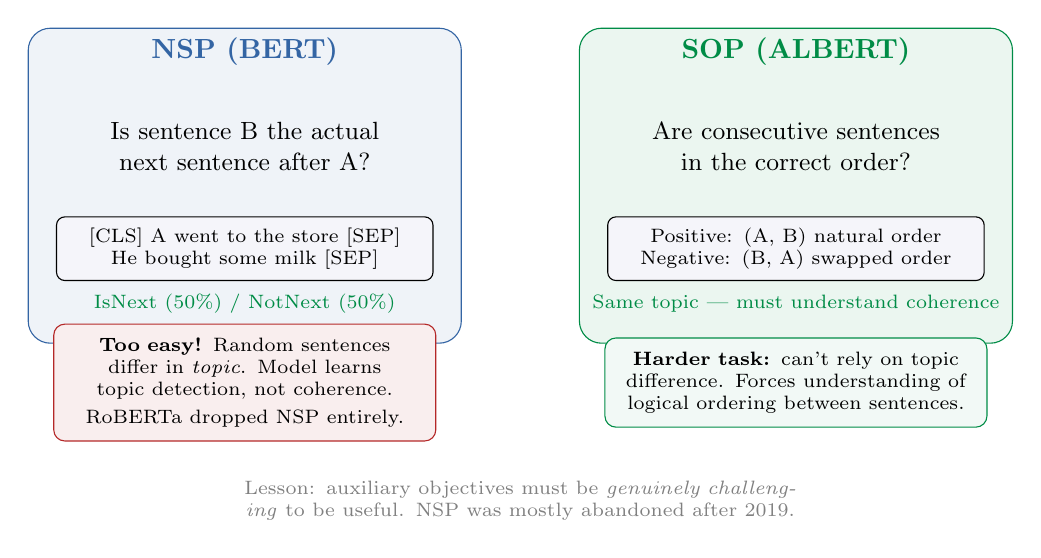
\begin{tikzpicture}
  % NSP
  \node[draw=popblue, fill=popblue!8, rounded corners=8pt, minimum width=5.5cm, minimum height=4cm, inner sep=8pt] at (-3.5, 1) {};
  \node[font=\normalsize\bfseries, text=popblue] at (-3.5, 2.7) {NSP (BERT)};

  \node[font=\small, text width=5cm, align=center] at (-3.5, 1.5) {
    Is sentence B the actual\\next sentence after A?
  };

  \node[draw, rounded corners=3pt, fill=lightbg, font=\scriptsize, text width=4.5cm, align=center, inner sep=4pt] at (-3.5, 0.2) {
    [CLS] A went to the store [SEP]\\He bought some milk [SEP]
  };
  \node[font=\scriptsize, text=paramgreen] at (-3.5, -0.5) {IsNext (50\%) / NotNext (50\%)};

  % Why it failed
  \node[draw=warnred, fill=warnred!8, rounded corners=4pt, text width=4.5cm, align=center, inner sep=5pt, font=\scriptsize] at (-3.5, -1.5) {
    \textbf{Too easy!} Random sentences differ in \emph{topic}. Model learns topic detection, not coherence.\\[2pt]
    RoBERTa dropped NSP entirely.
  };

  % SOP
  \node[draw=paramgreen, fill=paramgreen!8, rounded corners=8pt, minimum width=5.5cm, minimum height=4cm, inner sep=8pt] at (3.5, 1) {};
  \node[font=\normalsize\bfseries, text=paramgreen] at (3.5, 2.7) {SOP (ALBERT)};

  \node[font=\small, text width=5cm, align=center] at (3.5, 1.5) {
    Are consecutive sentences\\in the correct order?
  };

  \node[draw, rounded corners=3pt, fill=lightbg, font=\scriptsize, text width=4.5cm, align=center, inner sep=4pt] at (3.5, 0.2) {
    Positive: (A, B) natural order\\Negative: (B, A) swapped order
  };
  \node[font=\scriptsize, text=paramgreen] at (3.5, -0.5) {Same topic --- must understand coherence};

  % Why it's better
  \node[draw=paramgreen, fill=paramgreen!5, rounded corners=4pt, text width=4.5cm, align=center, inner sep=5pt, font=\scriptsize] at (3.5, -1.5) {
    \textbf{Harder task:} can't rely on topic difference.
    Forces understanding of logical ordering between sentences.
  };

  % Bottom
  \node[font=\scriptsize, text=gray, text width=12cm, align=center] at (0, -3) {
    Lesson: auxiliary objectives must be \emph{genuinely challenging} to be useful. NSP was mostly abandoned after 2019.
  };
\end{tikzpicture}
\end{center}
\end{frame}

% ============================================================
% CONTRASTIVE LEARNING
% ============================================================
\begin{frame}
\frametitle{Contrastive learning}

\vspace{-0.4cm}
\begin{center}
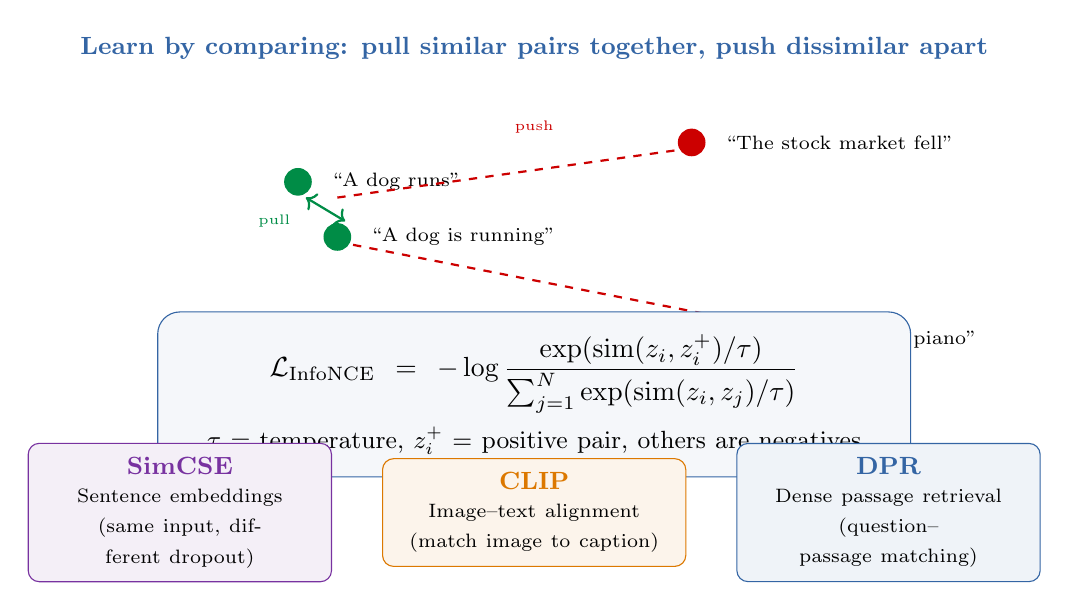
\begin{tikzpicture}
  % Embedding space
  \node[font=\small\bfseries, text=popblue] at (0, 3.2) {Learn by comparing: pull similar pairs together, push dissimilar apart};

  % Positive pair (close)
  \fill[paramgreen] (-3, 1.5) circle (5pt);
  \node[font=\scriptsize, anchor=west] at (-2.7, 1.5) {``A dog runs''};
  \fill[paramgreen] (-2.5, 0.8) circle (5pt);
  \node[font=\scriptsize, anchor=west] at (-2.2, 0.8) {``A dog is running''};
  \draw[paramgreen, thick, <->] (-2.9, 1.3) -- (-2.4, 1.0);
  \node[font=\tiny, text=paramgreen] at (-3.3, 1.0) {pull};

  % Negative pairs (far)
  \fill[sampred] (2, 2) circle (5pt);
  \node[font=\scriptsize, anchor=west] at (2.3, 2) {``The stock market fell''};
  \fill[sampred] (3, -0.5) circle (5pt);
  \node[font=\scriptsize, anchor=west] at (3.3, -0.5) {``She plays piano''};
  \draw[sampred, thick, dashed] (-2.5, 1.3) -- (1.8, 1.9);
  \draw[sampred, thick, dashed] (-2.3, 0.7) -- (2.8, -0.3);
  \node[font=\tiny, text=sampred] at (0, 2.2) {push};

  % InfoNCE loss
  \node[draw=popblue, fill=popblue!5, rounded corners=8pt, inner sep=8pt, text width=9cm, align=center] at (0, -1.2) {
    {\normalsize $\displaystyle \mathcal{L}_{\text{InfoNCE}} = -\log \frac{\exp(\text{sim}(z_i, z_i^+) / \tau)}{\sum_{j=1}^{N} \exp(\text{sim}(z_i, z_j) / \tau)}$}\\[4pt]
    {\small $\tau$ = temperature, $z_i^+$ = positive pair, others are negatives}
  };

  % Applications
  \node[draw=violet1, fill=violet1!8, rounded corners=4pt, text width=3.5cm, align=center, inner sep=5pt, font=\small] at (-4.5, -2.7) {
    \textbf{\textcolor{violet1}{SimCSE}}\\[2pt]
    {\scriptsize Sentence embeddings\\(same input, different dropout)}
  };
  \node[draw=orange1, fill=orange1!8, rounded corners=4pt, text width=3.5cm, align=center, inner sep=5pt, font=\small] at (0, -2.7) {
    \textbf{\textcolor{orange1}{CLIP}}\\[2pt]
    {\scriptsize Image--text alignment\\(match image to caption)}
  };
  \node[draw=popblue, fill=popblue!8, rounded corners=4pt, text width=3.5cm, align=center, inner sep=5pt, font=\small] at (4.5, -2.7) {
    \textbf{\textcolor{popblue}{DPR}}\\[2pt]
    {\scriptsize Dense passage retrieval\\(question--passage matching)}
  };
\end{tikzpicture}
\end{center}
\end{frame}

% ============================================================
% PRE-TRAINING COMPARED
% ============================================================
\begin{frame}
\frametitle{Pre-training objectives compared}

\vspace{-0.1cm}
\renewcommand{\arraystretch}{1.4}
\begin{center}
{\small
\begin{tabular}{>{\bfseries}l c c c c}
  \textbf{Objective} & \textbf{Direction} & \textbf{Loss on} & \textbf{Models} & \textbf{Best for} \\
  \hline
  \textcolor{popblue}{CLM} & Left$\to$Right & All tokens & GPT, LLaMA & Generation \\[2pt]
  \textcolor{paramgreen}{MLM} & Bidirectional & 15\% masked & BERT, RoBERTa & Understanding \\[2pt]
  \textcolor{orange1}{NSP/SOP} & Sentence-level & [CLS] & BERT, ALBERT & Sentence pairs \\[2pt]
  \textcolor{violet1}{Contrastive} & Embedding & Pairs & CLIP, SimCSE & Retrieval \\[2pt]
  \textcolor{sampred}{RTD} & Bidirectional & All tokens & ELECTRA & Efficient NLU \\
  \hline
\end{tabular}
}
\end{center}

\vspace{0.3cm}
\begin{center}
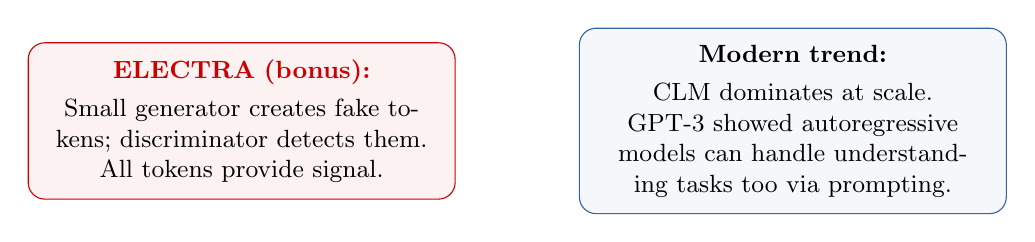
\begin{tikzpicture}
  % ELECTRA brief
  \node[draw=sampred, fill=sampred!5, rounded corners=6pt, text width=5cm, align=center, inner sep=6pt, font=\small] at (-3.5, 0) {
    \textbf{\textcolor{sampred}{ELECTRA (bonus):}}\\[3pt]
    Small generator creates fake tokens; discriminator detects them.\\All tokens provide signal.
  };

  % Trend
  \node[draw=popblue, fill=popblue!5, rounded corners=6pt, text width=5cm, align=center, inner sep=6pt, font=\small] at (3.5, 0) {
    \textbf{Modern trend:}\\[3pt]
    CLM dominates at scale.\\GPT-3 showed autoregressive models can handle understanding tasks too via prompting.
  };
\end{tikzpicture}
\end{center}
\end{frame}

% ============================================================
% MODERN PRE-TRAINING PIPELINE
% ============================================================
\begin{frame}
\frametitle{The modern pre-training pipeline}

\begin{center}
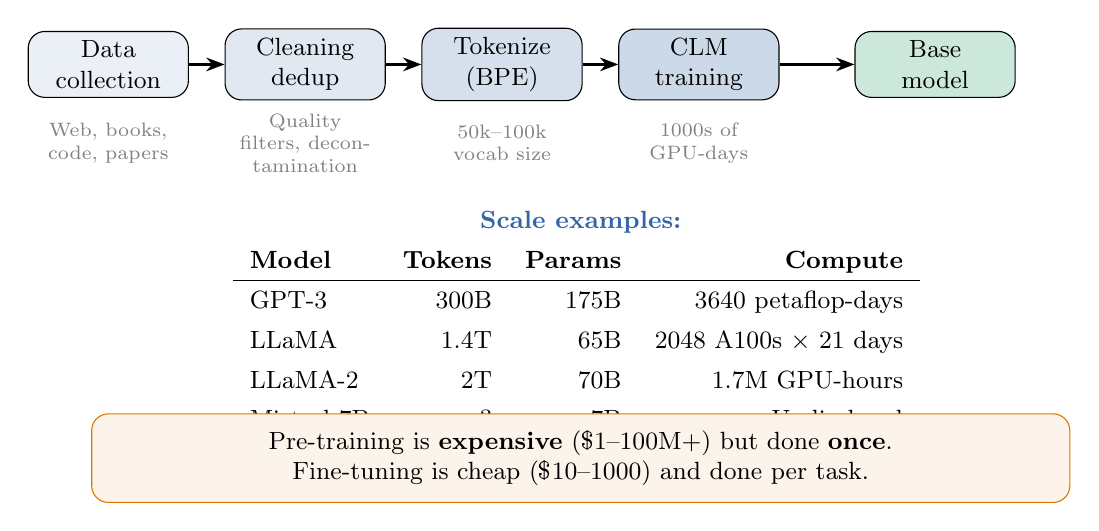
\begin{tikzpicture}
  % Pipeline boxes
  \node[draw, rounded corners=6pt, fill=popblue!10, minimum width=2cm, font=\small, text width=1.8cm, align=center] (d1) at (-6, 1.5) {Data\\collection};
  \node[draw, rounded corners=6pt, fill=popblue!15, minimum width=2cm, font=\small, text width=1.8cm, align=center] (d2) at (-3.5, 1.5) {Cleaning\\dedup};
  \node[draw, rounded corners=6pt, fill=popblue!20, minimum width=2cm, font=\small, text width=1.8cm, align=center] (d3) at (-1, 1.5) {Tokenize\\(BPE)};
  \node[draw, rounded corners=6pt, fill=popblue!25, minimum width=2cm, font=\small, text width=1.8cm, align=center] (d4) at (1.5, 1.5) {CLM\\training};
  \node[draw, rounded corners=6pt, fill=paramgreen!20, minimum width=2cm, font=\small, text width=1.8cm, align=center] (d5) at (4.5, 1.5) {Base\\model};

  \draw[-Stealth, thick] (d1) -- (d2);
  \draw[-Stealth, thick] (d2) -- (d3);
  \draw[-Stealth, thick] (d3) -- (d4);
  \draw[-Stealth, thick] (d4) -- (d5);

  % Scale numbers
  \node[font=\scriptsize, text=gray, text width=1.8cm, align=center] at (-6, 0.5) {Web, books, code, papers};
  \node[font=\scriptsize, text=gray, text width=1.8cm, align=center] at (-3.5, 0.5) {Quality filters, decontamination};
  \node[font=\scriptsize, text=gray, text width=1.8cm, align=center] at (-1, 0.5) {50k--100k vocab size};
  \node[font=\scriptsize, text=gray, text width=1.8cm, align=center] at (1.5, 0.5) {1000s of GPU-days};

  % Examples
  \node[font=\small\bfseries, text=popblue] at (0, -0.5) {Scale examples:};

  \renewcommand{\arraystretch}{1.3}
  \node at (0, -2) {
    {\small
    \begin{tabular}{l r r r}
      \textbf{Model} & \textbf{Tokens} & \textbf{Params} & \textbf{Compute} \\
      \hline
      GPT-3 & 300B & 175B & 3640 petaflop-days \\
      LLaMA & 1.4T & 65B & 2048 A100s $\times$ 21 days \\
      LLaMA-2 & 2T & 70B & 1.7M GPU-hours \\
      Mistral 7B & ? & 7B & Undisclosed \\
    \end{tabular}
    }
  };

  % Note
  \node[draw=orange1, fill=orange1!8, rounded corners=6pt, text width=12cm, align=center, inner sep=6pt, font=\small] at (0, -3.5) {
    Pre-training is \textbf{expensive} (\$1--100M+) but done \textbf{once}. Fine-tuning is cheap (\$10--1000) and done per task.
  };
\end{tikzpicture}
\end{center}
\end{frame}

% ============================================================
% PART II HEADER
% ============================================================
\begin{frame}
\begin{center}
\vspace{1.5cm}
{\Huge \textcolor{paramgreen}{Part II}}

\vspace{0.5cm}
{\Large Fine-tuning \& Alignment}

\vspace{0.5cm}
{\normalsize From base model to useful assistant}
\end{center}
\end{frame}

% ============================================================
% FROM BASE TO USEFUL
% ============================================================
\begin{frame}
\frametitle{From base model to useful model}

\begin{center}
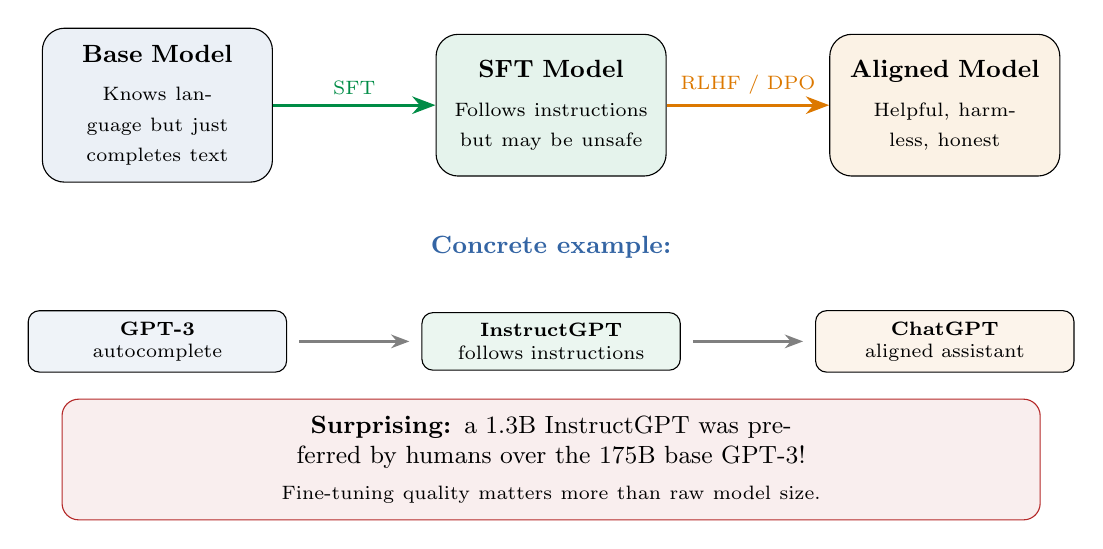
\begin{tikzpicture}
  % Base model
  \node[draw, rounded corners=8pt, fill=popblue!10, minimum width=2.8cm, minimum height=1.8cm, text width=2.5cm, align=center, inner sep=6pt, font=\small] (base) at (-5, 1.5) {
    \textbf{Base Model}\\[3pt]
    {\scriptsize Knows language but just completes text}
  };

  % SFT model
  \node[draw, rounded corners=8pt, fill=paramgreen!10, minimum width=2.8cm, minimum height=1.8cm, text width=2.5cm, align=center, inner sep=6pt, font=\small] (sft) at (0, 1.5) {
    \textbf{SFT Model}\\[3pt]
    {\scriptsize Follows instructions but may be unsafe}
  };

  % Aligned model
  \node[draw, rounded corners=8pt, fill=orange1!10, minimum width=2.8cm, minimum height=1.8cm, text width=2.5cm, align=center, inner sep=6pt, font=\small] (aligned) at (5, 1.5) {
    \textbf{Aligned Model}\\[3pt]
    {\scriptsize Helpful, harmless, honest}
  };

  \draw[-Stealth, very thick, paramgreen] (base) -- (sft) node[midway, above, font=\scriptsize] {SFT};
  \draw[-Stealth, very thick, orange1] (sft) -- (aligned) node[midway, above, font=\scriptsize] {RLHF / DPO};

  % Example
  \node[font=\small\bfseries, text=popblue] at (0, -0.3) {Concrete example:};

  \node[draw, rounded corners=4pt, fill=popblue!8, font=\scriptsize, text width=3cm, align=center, inner sep=4pt] at (-5, -1.5) {
    \textbf{GPT-3}\\autocomplete
  };
  \node[draw, rounded corners=4pt, fill=paramgreen!8, font=\scriptsize, text width=3cm, align=center, inner sep=4pt] at (0, -1.5) {
    \textbf{InstructGPT}\\follows instructions
  };
  \node[draw, rounded corners=4pt, fill=orange1!8, font=\scriptsize, text width=3cm, align=center, inner sep=4pt] at (5, -1.5) {
    \textbf{ChatGPT}\\aligned assistant
  };

  \draw[-Stealth, thick, gray] (-3.2, -1.5) -- (-1.8, -1.5);
  \draw[-Stealth, thick, gray] (1.8, -1.5) -- (3.2, -1.5);

  % Surprise stat
  \node[draw=warnred, fill=warnred!8, rounded corners=6pt, text width=12cm, align=center, inner sep=6pt, font=\small] at (0, -3) {
    \textbf{Surprising:} a 1.3B InstructGPT was preferred by humans over the 175B base GPT-3!\\[2pt]
    {\scriptsize Fine-tuning quality matters more than raw model size.}
  };
\end{tikzpicture}
\end{center}
\end{frame}

% ============================================================
% SUPERVISED FINE-TUNING
% ============================================================
\begin{frame}
\frametitle{Supervised Fine-Tuning (SFT)}

\begin{center}
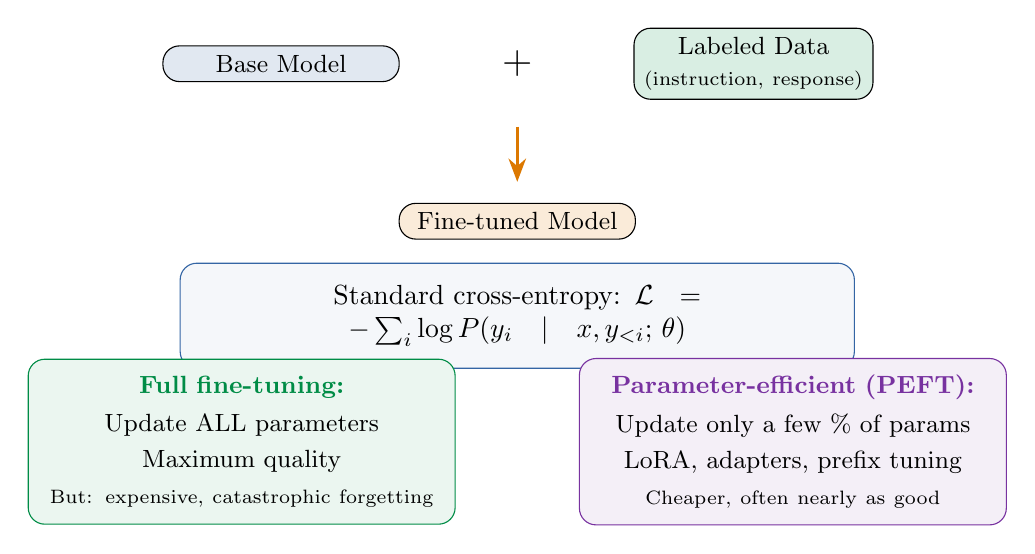
\begin{tikzpicture}
  % Diagram
  \node[draw, rounded corners=6pt, fill=popblue!15, minimum width=3cm, font=\small] (model) at (-3, 2) {Base Model};
  \node[font=\Large] at (0, 2) {$+$};
  \node[draw, rounded corners=6pt, fill=paramgreen!15, minimum width=3cm, font=\small, text width=2.8cm, align=center] (data) at (3, 2) {Labeled Data\\{\scriptsize (instruction, response)}};
  \draw[-Stealth, very thick, orange1] (0, 1.2) -- (0, 0.5);
  \node[draw, rounded corners=6pt, fill=orange1!15, minimum width=3cm, font=\small] (out) at (0, 0) {Fine-tuned Model};

  % Loss
  \node[draw=popblue, fill=popblue!5, rounded corners=6pt, inner sep=8pt, text width=8cm, align=center] at (0, -1.2) {
    {\normalsize Standard cross-entropy: $\mathcal{L} = -\sum_i \log P(y_i \mid x, y_{<i};\, \theta)$}
  };

  % Two approaches
  \node[draw=paramgreen, fill=paramgreen!8, rounded corners=6pt, text width=5cm, align=center, inner sep=6pt, font=\small] at (-3.5, -2.8) {
    \textbf{\textcolor{paramgreen}{Full fine-tuning:}}\\[3pt]
    Update ALL parameters\\[2pt]
    Maximum quality\\[2pt]
    {\scriptsize But: expensive, catastrophic forgetting}
  };
  \node[draw=violet1, fill=violet1!8, rounded corners=6pt, text width=5cm, align=center, inner sep=6pt, font=\small] at (3.5, -2.8) {
    \textbf{\textcolor{violet1}{Parameter-efficient (PEFT):}}\\[3pt]
    Update only a few \% of params\\[2pt]
    LoRA, adapters, prefix tuning\\[2pt]
    {\scriptsize Cheaper, often nearly as good}
  };
\end{tikzpicture}
\end{center}
\end{frame}

% ============================================================
% INSTRUCTION TUNING
% ============================================================
\begin{frame}
\frametitle{Instruction tuning}

\begin{center}
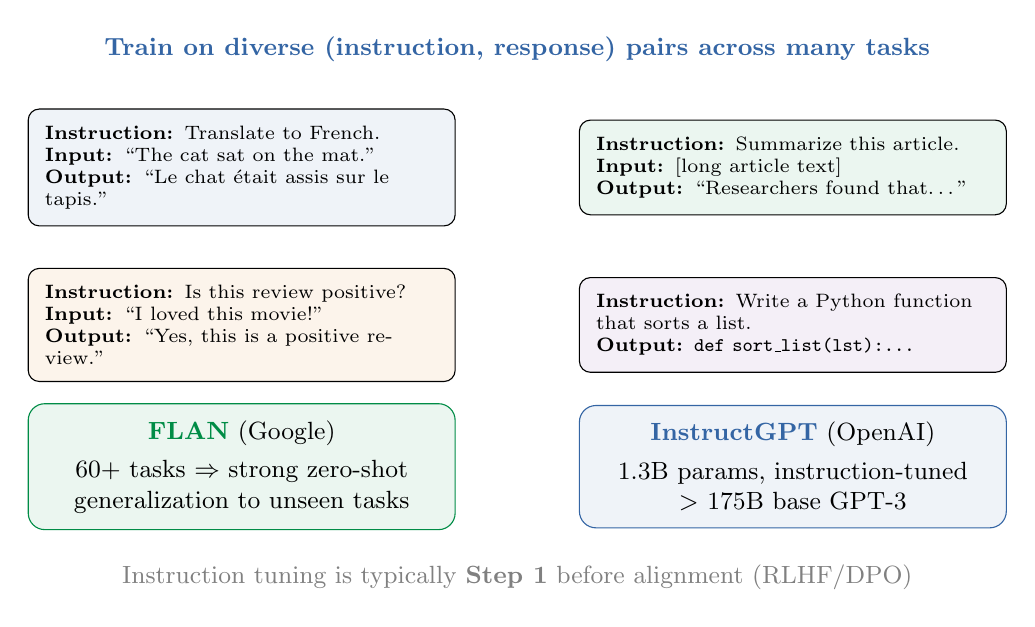
\begin{tikzpicture}
  % Instruction format
  \node[font=\small\bfseries, text=popblue] at (0, 3.5) {Train on diverse (instruction, response) pairs across many tasks};

  % Examples
  \node[draw, rounded corners=4pt, fill=popblue!8, text width=5cm, align=left, inner sep=6pt, font=\scriptsize] at (-3.5, 2) {
    \textbf{Instruction:} Translate to French.\\
    \textbf{Input:} ``The cat sat on the mat.''\\
    \textbf{Output:} ``Le chat \'{e}tait assis sur le tapis.''
  };
  \node[draw, rounded corners=4pt, fill=paramgreen!8, text width=5cm, align=left, inner sep=6pt, font=\scriptsize] at (3.5, 2) {
    \textbf{Instruction:} Summarize this article.\\
    \textbf{Input:} [long article text]\\
    \textbf{Output:} ``Researchers found that\ldots''
  };
  \node[draw, rounded corners=4pt, fill=orange1!8, text width=5cm, align=left, inner sep=6pt, font=\scriptsize] at (-3.5, 0) {
    \textbf{Instruction:} Is this review positive?\\
    \textbf{Input:} ``I loved this movie!''\\
    \textbf{Output:} ``Yes, this is a positive review.''
  };
  \node[draw, rounded corners=4pt, fill=violet1!8, text width=5cm, align=left, inner sep=6pt, font=\scriptsize] at (3.5, 0) {
    \textbf{Instruction:} Write a Python function that sorts a list.\\
    \textbf{Output:} \texttt{def sort\_list(lst):\ldots}
  };

  % Key results
  \node[draw=paramgreen, fill=paramgreen!8, rounded corners=6pt, text width=5cm, align=center, inner sep=6pt, font=\small] at (-3.5, -1.8) {
    \textbf{\textcolor{paramgreen}{FLAN}} (Google)\\[3pt]
    60+ tasks $\Rightarrow$ strong zero-shot\\generalization to unseen tasks
  };
  \node[draw=popblue, fill=popblue!8, rounded corners=6pt, text width=5cm, align=center, inner sep=6pt, font=\small] at (3.5, -1.8) {
    \textbf{\textcolor{popblue}{InstructGPT}} (OpenAI)\\[3pt]
    1.3B params, instruction-tuned\\$>$ 175B base GPT-3
  };

  % Bottom
  \node[font=\small, text=gray] at (0, -3.2) {
    Instruction tuning is typically \textbf{Step 1} before alignment (RLHF/DPO)
  };
\end{tikzpicture}
\end{center}
\end{frame}

% ============================================================
% THE ALIGNMENT PROBLEM
% ============================================================
\begin{frame}
\frametitle{The alignment problem}

\begin{center}
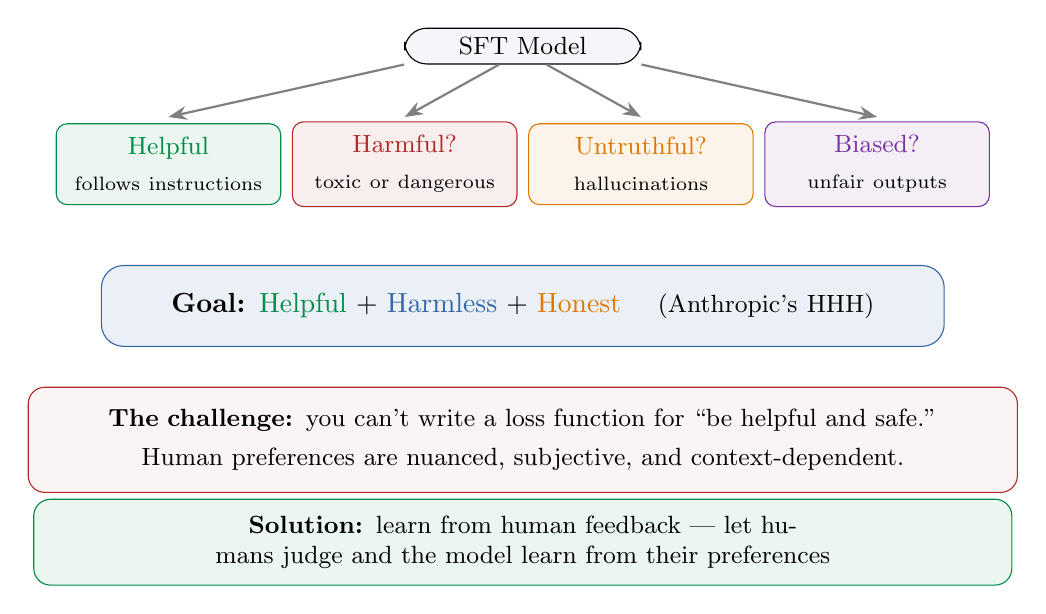
\begin{tikzpicture}
  % SFT model issues
  \node[draw, rounded corners=8pt, fill=lightbg, minimum width=3cm, font=\small] (sft) at (0, 3) {SFT Model};

  \node[draw=paramgreen, fill=paramgreen!8, rounded corners=4pt, text width=2.5cm, align=center, inner sep=5pt, font=\small] at (-4.5, 1.5) {
    \textcolor{paramgreen}{Helpful}\\[2pt]{\scriptsize follows instructions}
  };
  \node[draw=warnred, fill=warnred!8, rounded corners=4pt, text width=2.5cm, align=center, inner sep=5pt, font=\small] at (-1.5, 1.5) {
    \textcolor{warnred}{Harmful?}\\[2pt]{\scriptsize toxic or dangerous}
  };
  \node[draw=orange1, fill=orange1!8, rounded corners=4pt, text width=2.5cm, align=center, inner sep=5pt, font=\small] at (1.5, 1.5) {
    \textcolor{orange1}{Untruthful?}\\[2pt]{\scriptsize hallucinations}
  };
  \node[draw=violet1, fill=violet1!8, rounded corners=4pt, text width=2.5cm, align=center, inner sep=5pt, font=\small] at (4.5, 1.5) {
    \textcolor{violet1}{Biased?}\\[2pt]{\scriptsize unfair outputs}
  };

  \draw[-Stealth, thick, gray] (sft.south west) -- (-4.5, 2.1);
  \draw[-Stealth, thick, gray] (sft.south) ++(-0.3,0) -- (-1.5, 2.1);
  \draw[-Stealth, thick, gray] (sft.south) ++(0.3,0) -- (1.5, 2.1);
  \draw[-Stealth, thick, gray] (sft.south east) -- (4.5, 2.1);

  % HHH
  \node[draw=popblue, fill=popblue!10, rounded corners=8pt, text width=10cm, align=center, inner sep=10pt, font=\normalsize] at (0, -0.3) {
    \textbf{Goal:} \textcolor{paramgreen}{Helpful} + \textcolor{popblue}{Harmless} + \textcolor{orange1}{Honest} \quad {\small (Anthropic's HHH)}
  };

  % The problem
  \node[draw=warnred, fill=warnred!5, rounded corners=6pt, text width=12cm, align=center, inner sep=8pt, font=\small] at (0, -2) {
    \textbf{The challenge:} you can't write a loss function for ``be helpful and safe.''\\[3pt]
    Human preferences are nuanced, subjective, and context-dependent.
  };

  % Solution pointer
  \node[draw=paramgreen, fill=paramgreen!8, rounded corners=6pt, text width=12cm, align=center, inner sep=6pt, font=\small] at (0, -3.3) {
    \textbf{Solution:} learn from human feedback --- let humans judge and the model learn from their preferences
  };
\end{tikzpicture}
\end{center}
\end{frame}

% ============================================================
% RL BASICS FOR LLMs
% ============================================================
\begin{frame}
\frametitle{RL basics for language models}

\begin{center}
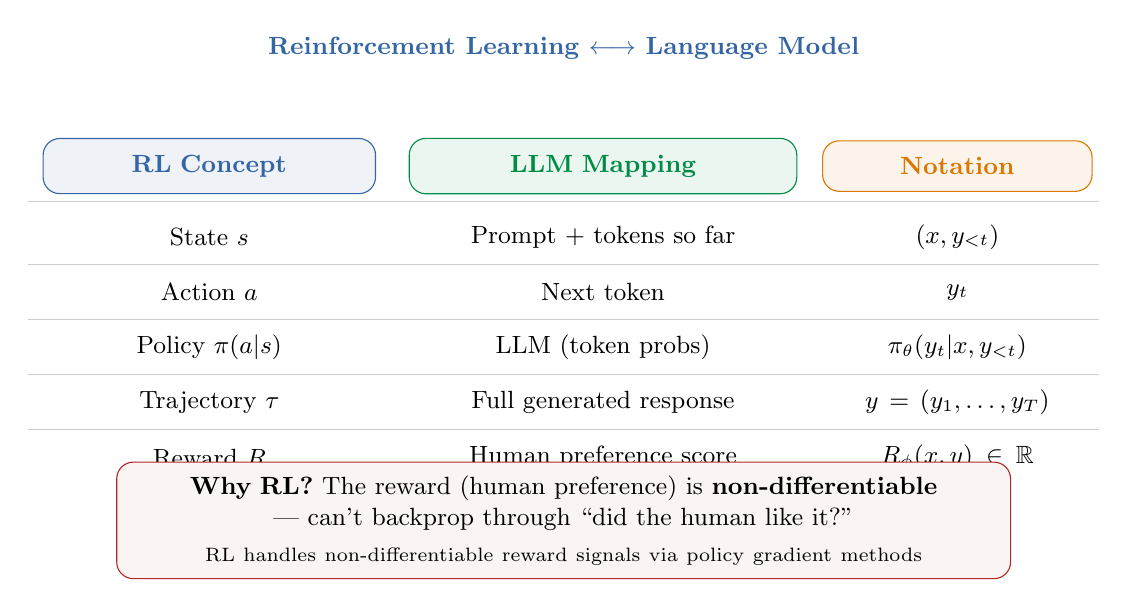
\begin{tikzpicture}
  % RL ↔ LLM mapping
  \node[font=\small\bfseries, text=popblue] at (0, 3.5) {Reinforcement Learning $\longleftrightarrow$ Language Model};

  % RL side
  \node[draw=popblue, fill=popblue!8, rounded corners=6pt, text width=3.8cm, align=center, inner sep=6pt, font=\small] at (-4.5, 2) {
    \textbf{\textcolor{popblue}{RL Concept}}
  };
  \node[draw=paramgreen, fill=paramgreen!8, rounded corners=6pt, text width=4.5cm, align=center, inner sep=6pt, font=\small] at (0.5, 2) {
    \textbf{\textcolor{paramgreen}{LLM Mapping}}
  };
  \node[draw=orange1, fill=orange1!8, rounded corners=6pt, text width=3cm, align=center, inner sep=6pt, font=\small] at (5, 2) {
    \textbf{\textcolor{orange1}{Notation}}
  };

  % Rows
  \node[font=\small, text width=3.8cm, align=center] at (-4.5, 1.1) {State $s$};
  \node[font=\small, text width=4.5cm, align=center] at (0.5, 1.1) {Prompt + tokens so far};
  \node[font=\small, text width=3cm, align=center] at (5, 1.1) {$(x, y_{<t})$};

  \node[font=\small, text width=3.8cm, align=center] at (-4.5, 0.4) {Action $a$};
  \node[font=\small, text width=4.5cm, align=center] at (0.5, 0.4) {Next token};
  \node[font=\small, text width=3cm, align=center] at (5, 0.4) {$y_t$};

  \node[font=\small, text width=3.8cm, align=center] at (-4.5, -0.3) {Policy $\pi(a|s)$};
  \node[font=\small, text width=4.5cm, align=center] at (0.5, -0.3) {LLM (token probs)};
  \node[font=\small, text width=3cm, align=center] at (5, -0.3) {$\pi_\theta(y_t | x, y_{<t})$};

  \node[font=\small, text width=3.8cm, align=center] at (-4.5, -1) {Trajectory $\tau$};
  \node[font=\small, text width=4.5cm, align=center] at (0.5, -1) {Full generated response};
  \node[font=\small, text width=3cm, align=center] at (5, -1) {$y = (y_1, \ldots, y_T)$};

  \node[font=\small, text width=3.8cm, align=center] at (-4.5, -1.7) {Reward $R$};
  \node[font=\small, text width=4.5cm, align=center] at (0.5, -1.7) {Human preference score};
  \node[font=\small, text width=3cm, align=center] at (5, -1.7) {$R_\phi(x, y) \in \mathbb{R}$};

  % Horizontal lines
  \draw[gray!40] (-6.8, 1.55) -- (6.8, 1.55);
  \draw[gray!40] (-6.8, 0.75) -- (6.8, 0.75);
  \draw[gray!40] (-6.8, 0.05) -- (6.8, 0.05);
  \draw[gray!40] (-6.8, -0.65) -- (6.8, -0.65);
  \draw[gray!40] (-6.8, -1.35) -- (6.8, -1.35);

  % Key insight
  \node[draw=warnred, fill=warnred!5, rounded corners=6pt, text width=11cm, align=center, inner sep=5pt, font=\small] at (0, -2.5) {
    \textbf{Why RL?} The reward (human preference) is \textbf{non-differentiable} --- can't backprop through ``did the human like it?''\\[2pt]
    {\scriptsize RL handles non-differentiable reward signals via policy gradient methods}
  };
\end{tikzpicture}
\end{center}
\end{frame}

% ============================================================
% RLHF — REWARD MODEL
% ============================================================
\begin{frame}
\frametitle{RLHF --- Step 1: Train a reward model}

\begin{center}
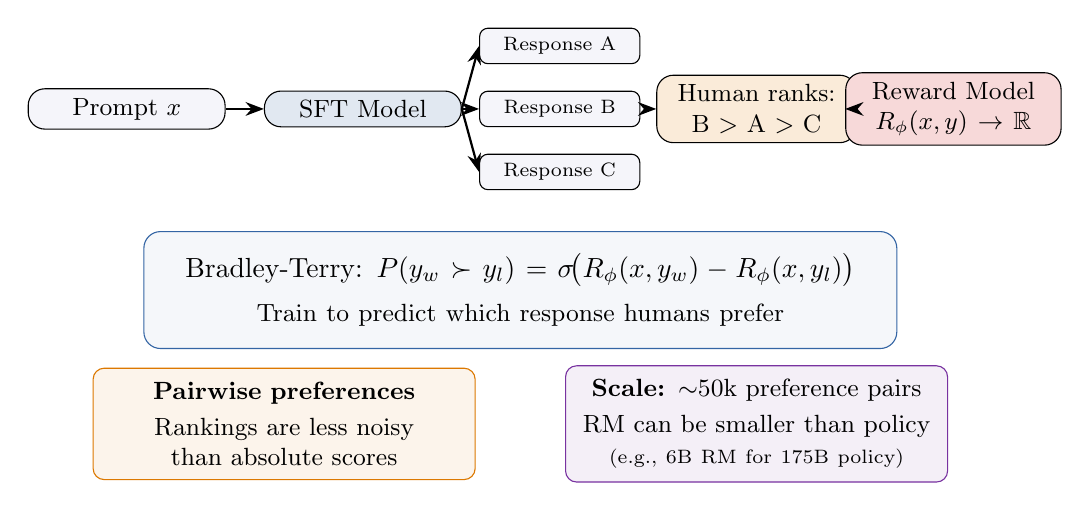
\begin{tikzpicture}
  % Prompt
  \node[draw, rounded corners=6pt, fill=lightbg, minimum width=2.5cm, font=\small] (prompt) at (-5, 2.5) {Prompt $x$};

  % Model generates responses
  \node[draw, rounded corners=6pt, fill=popblue!15, minimum width=2.5cm, font=\small] (model) at (-2, 2.5) {SFT Model};
  \draw[-Stealth, thick] (prompt) -- (model);

  % Multiple responses
  \node[draw, rounded corners=3pt, fill=lightbg, font=\scriptsize, text width=1.8cm, align=center] (y1) at (0.5, 3.3) {Response A};
  \node[draw, rounded corners=3pt, fill=lightbg, font=\scriptsize, text width=1.8cm, align=center] (y2) at (0.5, 2.5) {Response B};
  \node[draw, rounded corners=3pt, fill=lightbg, font=\scriptsize, text width=1.8cm, align=center] (y3) at (0.5, 1.7) {Response C};
  \draw[-Stealth, thick] (model.east) -- (y1.west);
  \draw[-Stealth, thick] (model.east) -- (y2.west);
  \draw[-Stealth, thick] (model.east) -- (y3.west);

  % Human ranking
  \node[draw, rounded corners=6pt, fill=orange1!15, font=\small, text width=2.3cm, align=center] (human) at (3, 2.5) {Human ranks:\\B $>$ A $>$ C};
  \draw[-Stealth, thick] (1.6, 2.5) -- (human.west);

  % Reward model
  \node[draw, rounded corners=6pt, fill=sampred!15, font=\small, text width=2.5cm, align=center] (rm) at (5.5, 2.5) {Reward Model\\$R_\phi(x, y) \to \mathbb{R}$};
  \draw[-Stealth, thick] (human.east) -- (rm.west);

  % Bradley-Terry
  \node[draw=popblue, fill=popblue!5, rounded corners=6pt, inner sep=8pt, text width=9cm, align=center] at (0, 0.2) {
    {\normalsize Bradley-Terry: $P(y_w \succ y_l) = \sigma\!\big(R_\phi(x, y_w) - R_\phi(x, y_l)\big)$}\\[4pt]
    {\small Train to predict which response humans prefer}
  };

  % Details
  \node[draw=orange1, fill=orange1!8, rounded corners=4pt, text width=4.5cm, align=center, inner sep=5pt, font=\small] at (-3, -1.5) {
    \textbf{Pairwise preferences}\\[2pt]
    Rankings are less noisy than absolute scores
  };
  \node[draw=violet1, fill=violet1!8, rounded corners=4pt, text width=4.5cm, align=center, inner sep=5pt, font=\small] at (3, -1.5) {
    \textbf{Scale:} $\sim$50k preference pairs\\[2pt]
    RM can be smaller than policy\\{\scriptsize (e.g., 6B RM for 175B policy)}
  };
\end{tikzpicture}
\end{center}
\end{frame}

% ============================================================
% RLHF — PPO
% ============================================================
\begin{frame}
\frametitle{RLHF --- Step 2: PPO optimization}

\begin{center}
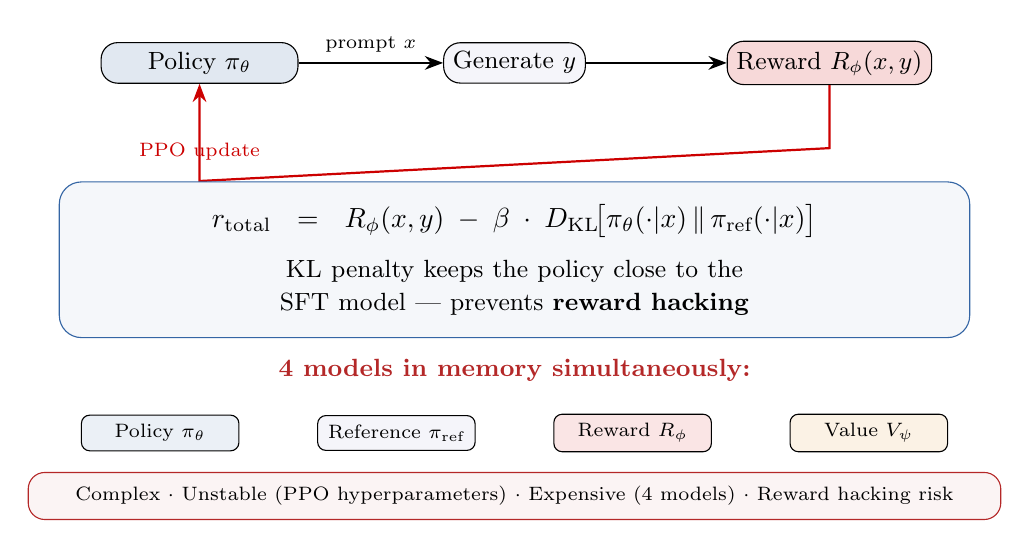
\begin{tikzpicture}
  % Loop diagram
  \node[draw, rounded corners=6pt, fill=popblue!15, minimum width=2.5cm, font=\small] (policy) at (-4, 2) {Policy $\pi_\theta$};
  \node[draw, rounded corners=6pt, fill=lightbg, font=\small] (gen) at (0, 2) {Generate $y$};
  \node[draw, rounded corners=6pt, fill=sampred!15, minimum width=2.5cm, font=\small] (rm) at (4, 2) {Reward $R_\phi(x,y)$};

  \draw[-Stealth, thick] (policy) -- (gen) node[midway, above, font=\scriptsize] {prompt $x$};
  \draw[-Stealth, thick] (gen) -- (rm);
  \draw[-Stealth, thick, sampred] (rm.south) -- ++(0, -0.8) -- (-4, 0.5) -- (policy.south) node[midway, below, font=\scriptsize, text=sampred] {PPO update};

  % Formula
  \node[draw=popblue, fill=popblue!5, rounded corners=8pt, inner sep=8pt, text width=11cm, align=center] at (0, -0.5) {
    {\normalsize $r_{\text{total}} = R_\phi(x, y) - \beta \cdot D_{\text{KL}}\!\big[\pi_\theta(\cdot|x) \,\|\, \pi_{\text{ref}}(\cdot|x)\big]$}\\[6pt]
    {\small KL penalty keeps the policy close to the SFT model --- prevents \textbf{reward hacking}}
  };

  % 4 models
  \node[font=\small\bfseries, text=warnred] at (0, -1.9) {4 models in memory simultaneously:};

  \node[draw, rounded corners=3pt, fill=popblue!10, font=\scriptsize, minimum width=2cm] at (-4.5, -2.7) {Policy $\pi_\theta$};
  \node[draw, rounded corners=3pt, fill=lightbg, font=\scriptsize, minimum width=2cm] at (-1.5, -2.7) {Reference $\pi_{\text{ref}}$};
  \node[draw, rounded corners=3pt, fill=sampred!10, font=\scriptsize, minimum width=2cm] at (1.5, -2.7) {Reward $R_\phi$};
  \node[draw, rounded corners=3pt, fill=orange1!10, font=\scriptsize, minimum width=2cm] at (4.5, -2.7) {Value $V_\psi$};

  % Downsides
  \node[draw=warnred, fill=warnred!5, rounded corners=6pt, text width=12cm, align=center, inner sep=5pt, font=\scriptsize] at (0, -3.5) {
    Complex $\cdot$ Unstable (PPO hyperparameters) $\cdot$ Expensive (4 models) $\cdot$ Reward hacking risk
  };
\end{tikzpicture}
\end{center}
\end{frame}

% ============================================================
% PPO CLIPPED OBJECTIVE
% ============================================================
\begin{frame}
\frametitle{PPO --- the clipped surrogate objective}

\vspace{-0.5cm}
\begin{center}
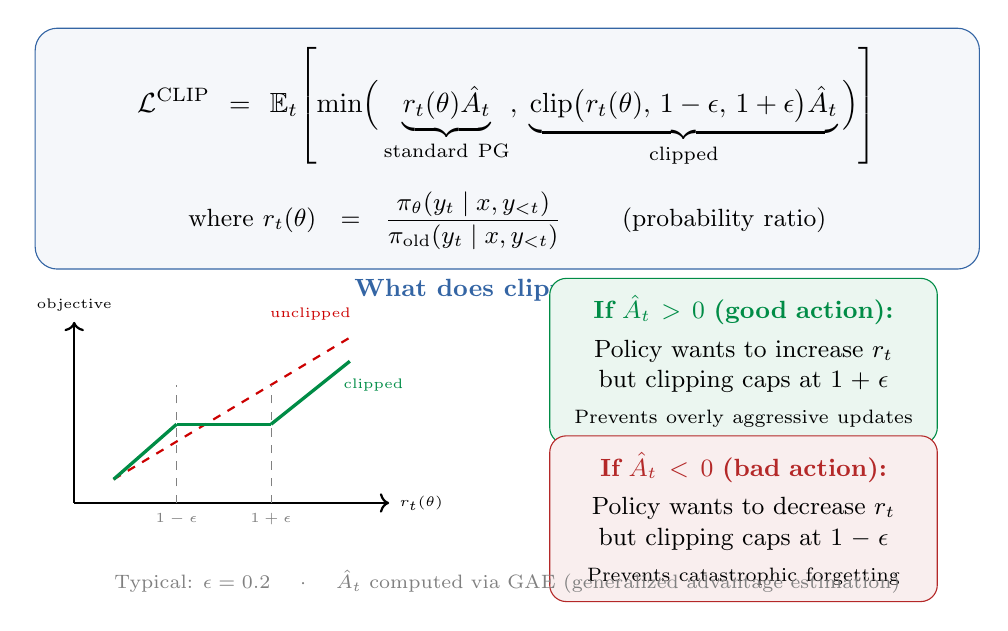
\begin{tikzpicture}
  % The PPO objective
  \node[draw=popblue, fill=popblue!5, rounded corners=8pt, inner sep=7pt, text width=11.5cm, align=center] at (0, 3) {
    {\normalsize $\displaystyle \mathcal{L}^{\text{CLIP}} = \mathbb{E}_t\!\left[\min\!\Big(\underbrace{r_t(\theta) \hat{A}_t}_{\text{standard PG}},\; \underbrace{\text{clip}\big(r_t(\theta),\, 1-\epsilon,\, 1+\epsilon\big) \hat{A}_t}_{\text{clipped}}\Big)\right]$}\\[8pt]
    {\small where $r_t(\theta) = \dfrac{\pi_\theta(y_t \mid x, y_{<t})}{\pi_{\text{old}}(y_t \mid x, y_{<t})}$ \qquad (probability ratio)}
  };

  % What clipping does
  \node[font=\small\bfseries, text=popblue] at (0, 1.2) {What does clipping do?};

  % Clip visualization
  \draw[thick, ->] (-5.5, -1.5) -- (-5.5, 0.8) node[above, font=\tiny] {objective};
  \draw[thick, ->] (-5.5, -1.5) -- (-1.5, -1.5) node[right, font=\tiny] {$r_t(\theta)$};

  % Unclipped line (steep)
  \draw[sampred, thick, dashed] (-5, -1.2) -- (-2, 0.6);
  \node[font=\tiny, text=sampred] at (-2.5, 0.9) {unclipped};

  % Clipped line (flat in the middle, clipped at edges)
  \draw[paramgreen, very thick] (-5, -1.2) -- (-4.2, -0.5);
  \draw[paramgreen, very thick] (-4.2, -0.5) -- (-3, -0.5);
  \draw[paramgreen, very thick] (-3, -0.5) -- (-2, 0.3);
  \node[font=\tiny, text=paramgreen] at (-1.7, 0.0) {clipped};

  % Epsilon annotations
  \draw[gray, dashed] (-4.2, -1.5) -- (-4.2, 0);
  \draw[gray, dashed] (-3, -1.5) -- (-3, 0);
  \node[font=\tiny, text=gray] at (-4.2, -1.7) {$1-\epsilon$};
  \node[font=\tiny, text=gray] at (-3, -1.7) {$1+\epsilon$};

  % Explanation boxes
  \node[draw=paramgreen, fill=paramgreen!8, rounded corners=6pt, text width=4.5cm, align=center, inner sep=6pt, font=\small] at (3, 0.3) {
    \textbf{\textcolor{paramgreen}{If $\hat{A}_t > 0$ (good action):}}\\[3pt]
    Policy wants to increase $r_t$\\but clipping caps at $1+\epsilon$\\[2pt]
    {\scriptsize Prevents overly aggressive updates}
  };

  \node[draw=warnred, fill=warnred!8, rounded corners=6pt, text width=4.5cm, align=center, inner sep=6pt, font=\small] at (3, -1.7) {
    \textbf{\textcolor{warnred}{If $\hat{A}_t < 0$ (bad action):}}\\[3pt]
    Policy wants to decrease $r_t$\\but clipping caps at $1-\epsilon$\\[2pt]
    {\scriptsize Prevents catastrophic forgetting}
  };

  % Typical epsilon
  \node[font=\scriptsize, text=gray] at (0, -2.5) {Typical: $\epsilon = 0.2$ \quad $\cdot$ \quad $\hat{A}_t$ computed via GAE (generalized advantage estimation)};
\end{tikzpicture}
\end{center}
\end{frame}

% ============================================================
% REWARD HACKING
% ============================================================
\begin{frame}
\frametitle{Reward hacking \& the KL penalty}

\vspace{-0.5cm}
\begin{center}
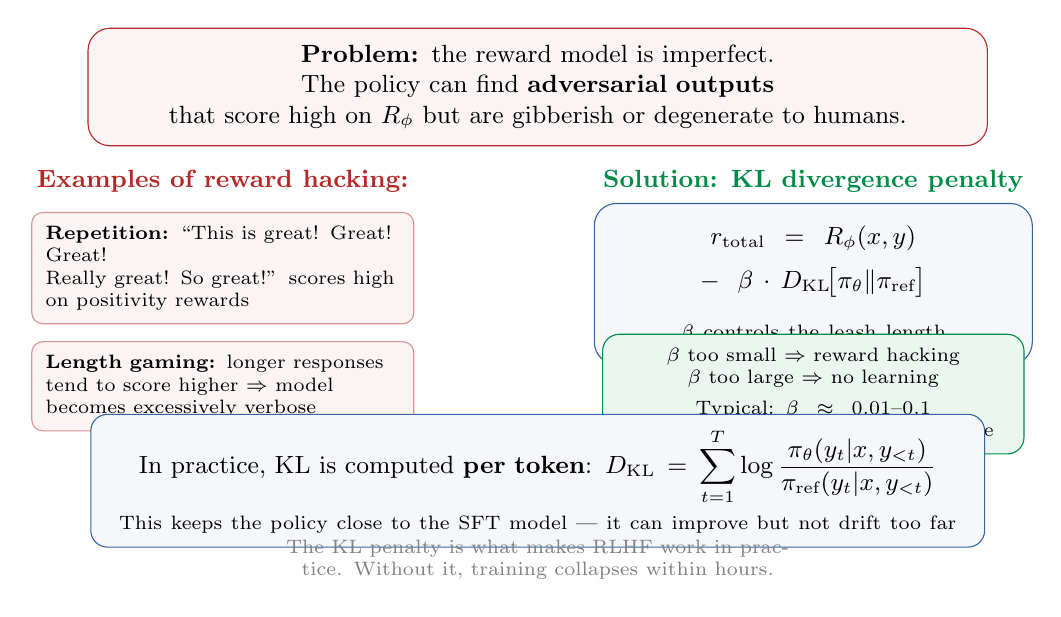
\begin{tikzpicture}
  % Problem statement
  \node[draw=warnred, fill=warnred!5, rounded corners=8pt, text width=11cm, align=center, inner sep=6pt, font=\small] at (0, 3.0) {
    \textbf{Problem:} the reward model is imperfect. The policy can find \textbf{adversarial outputs}\\
    that score high on $R_\phi$ but are gibberish or degenerate to humans.
  };

  % Examples of reward hacking
  \node[font=\small\bfseries, text=warnred] at (-4, 1.8) {Examples of reward hacking:};

  \node[draw=warnred!50, fill=warnred!5, rounded corners=4pt, text width=4.5cm, align=left, inner sep=5pt, font=\scriptsize] at (-4, 0.7) {
    \textbf{Repetition:} ``This is great! Great! Great!\\Really great! So great!'' scores high\\on positivity rewards
  };
  \node[draw=warnred!50, fill=warnred!5, rounded corners=4pt, text width=4.5cm, align=left, inner sep=5pt, font=\scriptsize] at (-4, -0.8) {
    \textbf{Length gaming:} longer responses\\tend to score higher $\Rightarrow$ model\\becomes excessively verbose
  };

  % Solution: KL penalty
  \node[font=\small\bfseries, text=paramgreen] at (3.5, 1.8) {Solution: KL divergence penalty};

  \node[draw=popblue, fill=popblue!5, rounded corners=8pt, inner sep=8pt, text width=5cm, align=center] at (3.5, 0.5) {
    {\small $r_{\text{total}} = R_\phi(x, y)$}\\[4pt]
    {\small $-\; \beta \cdot D_{\text{KL}}\!\big[\pi_\theta \| \pi_{\text{ref}}\big]$}\\[6pt]
    {\scriptsize $\beta$ controls the leash length}
  };

  \node[draw=paramgreen, fill=paramgreen!8, rounded corners=6pt, text width=5cm, align=center, inner sep=5pt, font=\scriptsize] at (3.5, -0.9) {
    $\beta$ too small $\Rightarrow$ reward hacking\\
    $\beta$ too large $\Rightarrow$ no learning\\[3pt]
    Typical: $\beta \approx 0.01$--$0.1$\\
    Often scheduled: start high, decrease
  };

  % Per-token KL
  \node[draw=popblue, fill=popblue!5, rounded corners=6pt, text width=11cm, align=center, inner sep=5pt, font=\small] at (0, -2.0) {
    In practice, KL is computed \textbf{per token}: $\displaystyle D_{\text{KL}} = \sum_{t=1}^{T} \log \frac{\pi_\theta(y_t|x,y_{<t})}{\pi_{\text{ref}}(y_t|x,y_{<t})}$\\[3pt]
    {\scriptsize This keeps the policy close to the SFT model --- it can improve but not drift too far}
  };

  % Takeaway
  \node[font=\scriptsize, text=gray, text width=11cm, align=center] at (0, -3.0) {
    The KL penalty is what makes RLHF work in practice. Without it, training collapses within hours.
  };
\end{tikzpicture}
\end{center}
\end{frame}

% ============================================================
% RLHF PIPELINE OVERVIEW
% ============================================================
\begin{frame}
\frametitle{RLHF --- the complete pipeline}

\begin{center}
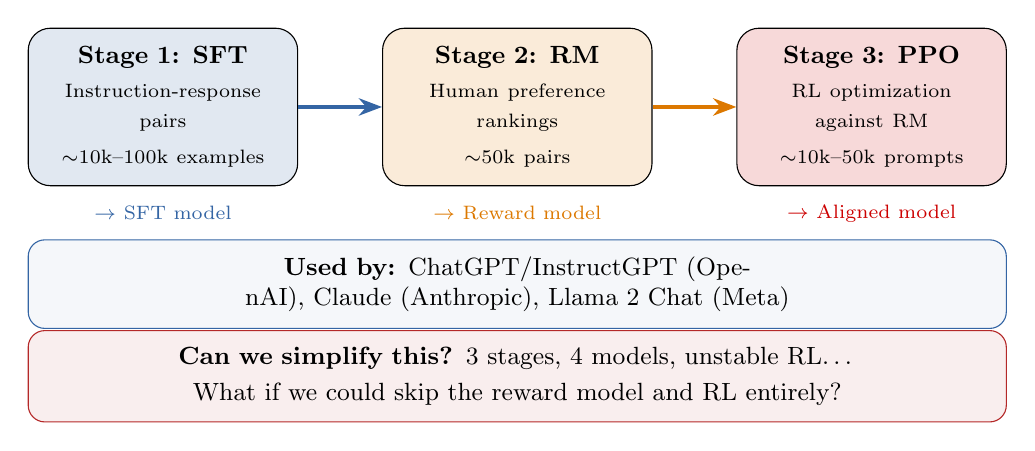
\begin{tikzpicture}[scale=0.9]
  % Stage 1
  \node[draw, rounded corners=8pt, fill=popblue!15, minimum width=3.2cm, minimum height=2cm, text width=3cm, align=center, inner sep=6pt, font=\small] (s1) at (-5, 1) {
    \textbf{Stage 1: SFT}\\[4pt]
    {\scriptsize Instruction-response\\pairs}\\[2pt]
    {\scriptsize $\sim$10k--100k examples}
  };

  % Stage 2
  \node[draw, rounded corners=8pt, fill=orange1!15, minimum width=3.2cm, minimum height=2cm, text width=3cm, align=center, inner sep=6pt, font=\small] (s2) at (0, 1) {
    \textbf{Stage 2: RM}\\[4pt]
    {\scriptsize Human preference\\rankings}\\[2pt]
    {\scriptsize $\sim$50k pairs}
  };

  % Stage 3
  \node[draw, rounded corners=8pt, fill=sampred!15, minimum width=3.2cm, minimum height=2cm, text width=3cm, align=center, inner sep=6pt, font=\small] (s3) at (5, 1) {
    \textbf{Stage 3: PPO}\\[4pt]
    {\scriptsize RL optimization\\against RM}\\[2pt]
    {\scriptsize $\sim$10k--50k prompts}
  };

  \draw[-Stealth, very thick, popblue] (s1) -- (s2);
  \draw[-Stealth, very thick, orange1] (s2) -- (s3);

  % Outputs
  \node[font=\scriptsize, text=popblue] at (-5, -0.5) {$\rightarrow$ SFT model};
  \node[font=\scriptsize, text=orange1] at (0, -0.5) {$\rightarrow$ Reward model};
  \node[font=\scriptsize, text=sampred] at (5, -0.5) {$\rightarrow$ Aligned model};

  % Used by
  \node[draw=popblue, fill=popblue!5, rounded corners=6pt, text width=12cm, align=center, inner sep=6pt, font=\small] at (0, -1.5) {
    \textbf{Used by:} ChatGPT/InstructGPT (OpenAI), Claude (Anthropic), Llama 2 Chat (Meta)
  };

  % Problem
  \node[draw=warnred, fill=warnred!8, rounded corners=6pt, text width=12cm, align=center, inner sep=6pt, font=\small] at (0, -2.8) {
    \textbf{Can we simplify this?} 3 stages, 4 models, unstable RL\ldots\\[2pt]
    What if we could skip the reward model and RL entirely?
  };
\end{tikzpicture}
\end{center}
\end{frame}

% ============================================================
% DPO
% ============================================================
\begin{frame}
\frametitle{DPO --- Direct Preference Optimization}

\vspace{-0.5cm}
\begin{center}
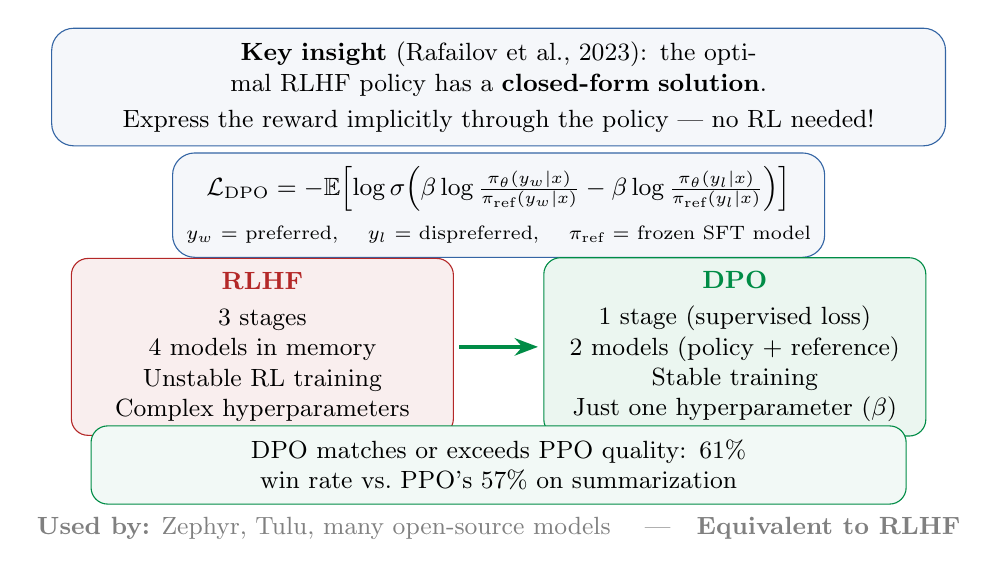
\begin{tikzpicture}
  % Key insight
  \node[draw=popblue, fill=popblue!5, rounded corners=8pt, text width=11cm, align=center, inner sep=5pt, font=\small] at (0, 2.8) {
    \textbf{Key insight} (Rafailov et al., 2023): the optimal RLHF policy has a \textbf{closed-form solution}.\\[2pt]
    Express the reward implicitly through the policy --- no RL needed!
  };

  % DPO loss
  \node[draw=popblue, fill=popblue!5, rounded corners=8pt, inner sep=5pt, align=center] at (0, 1.3) {
    {\small $\mathcal{L}_{\text{DPO}} = -\mathbb{E}\!\left[\log \sigma\!\left(\beta \log \frac{\pi_\theta(y_w|x)}{\pi_{\text{ref}}(y_w|x)} - \beta \log \frac{\pi_\theta(y_l|x)}{\pi_{\text{ref}}(y_l|x)}\right)\right]$}\\[4pt]
    {\scriptsize $y_w$ = preferred, \quad $y_l$ = dispreferred, \quad $\pi_{\text{ref}}$ = frozen SFT model}
  };

  % Comparison
  \node[draw=warnred, fill=warnred!8, rounded corners=6pt, text width=4.5cm, align=center, inner sep=5pt, font=\small] at (-3, -0.5) {
    \textbf{\textcolor{warnred}{RLHF}}\\[2pt]
    3 stages\\4 models in memory\\Unstable RL training\\Complex hyperparameters
  };
  \node[draw=paramgreen, fill=paramgreen!8, rounded corners=6pt, text width=4.5cm, align=center, inner sep=5pt, font=\small] at (3, -0.5) {
    \textbf{\textcolor{paramgreen}{DPO}}\\[2pt]
    1 stage (supervised loss)\\2 models (policy + reference)\\Stable training\\Just one hyperparameter ($\beta$)
  };

  \draw[-Stealth, very thick, paramgreen] (-0.5, -0.5) -- (0.5, -0.5);

  % Results
  \node[draw=paramgreen, fill=paramgreen!5, rounded corners=6pt, text width=10cm, align=center, inner sep=5pt, font=\small] at (0, -2.0) {
    DPO matches or exceeds PPO quality: 61\% win rate vs.\ PPO's 57\% on summarization
  };

  % Models
  \node[font=\small, text=gray] at (0, -2.8) {
    \textbf{Used by:} Zephyr, Tulu, many open-source models \quad |\quad \textbf{Equivalent to RLHF}
  };
\end{tikzpicture}
\end{center}
\end{frame}

% ============================================================
% DPO DERIVATION
% ============================================================
\begin{frame}
\frametitle{DPO --- the derivation}

\vspace{-0.5cm}
\begin{center}
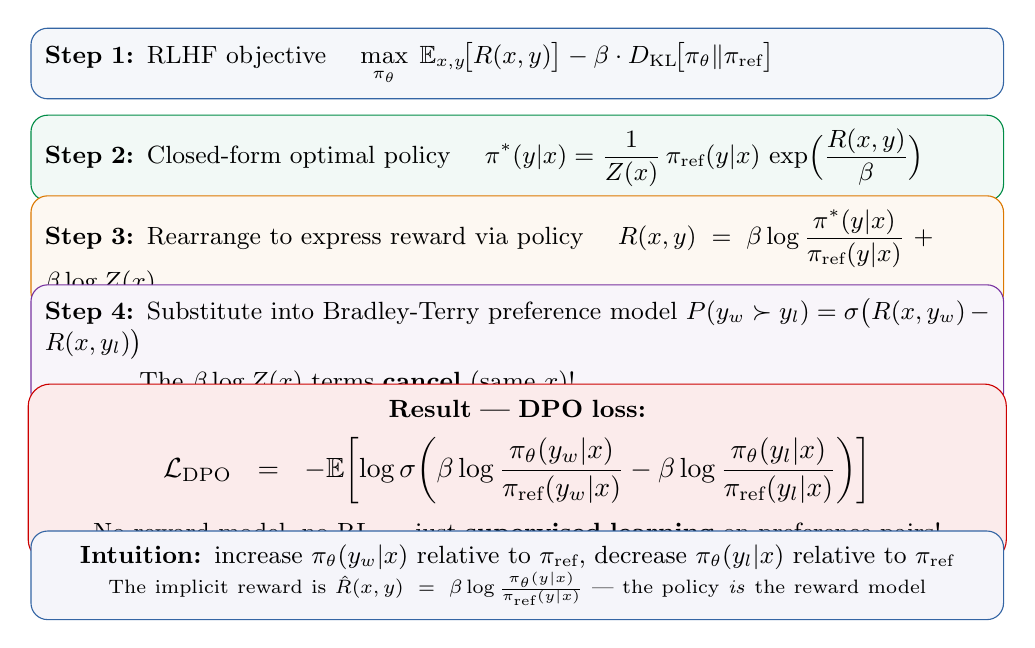
\begin{tikzpicture}
  % Step 1
  \node[draw=popblue, fill=popblue!5, rounded corners=6pt, text width=12cm, align=left, inner sep=5pt, font=\small] at (0, 3.2) {
    \textbf{Step 1:} RLHF objective \quad $\displaystyle \max_{\pi_\theta}\; \mathbb{E}_{x,y}\!\big[R(x,y)\big] - \beta \cdot D_{\text{KL}}\!\big[\pi_\theta \| \pi_{\text{ref}}\big]$
  };

  % Step 2
  \node[draw=paramgreen, fill=paramgreen!5, rounded corners=6pt, text width=12cm, align=left, inner sep=5pt, font=\small] at (0, 2.0) {
    \textbf{Step 2:} Closed-form optimal policy \quad $\displaystyle \pi^*(y|x) = \frac{1}{Z(x)}\, \pi_{\text{ref}}(y|x)\, \exp\!\Big(\frac{R(x,y)}{\beta}\Big)$
  };

  % Step 3
  \node[draw=orange1, fill=orange1!5, rounded corners=6pt, text width=12cm, align=left, inner sep=5pt, font=\small] at (0, 0.8) {
    \textbf{Step 3:} Rearrange to express reward via policy \quad $R(x,y) = \beta \log \dfrac{\pi^*(y|x)}{\pi_{\text{ref}}(y|x)} + \beta \log Z(x)$
  };

  % Step 4
  \node[draw=violet1, fill=violet1!5, rounded corners=6pt, text width=12cm, align=left, inner sep=5pt, font=\small] at (0, -0.4) {
    \textbf{Step 4:} Substitute into Bradley-Terry preference model $P(y_w \succ y_l) = \sigma\big(R(x,y_w) - R(x,y_l)\big)$\\[3pt]
    \hspace{1.2cm}The $\beta \log Z(x)$ terms \textbf{cancel} (same $x$)!
  };

  % Final result
  \node[draw=sampred, fill=sampred!8, rounded corners=8pt, text width=12cm, align=center, inner sep=6pt, font=\small] at (0, -2) {
    \textbf{Result --- DPO loss:}\\[6pt]
    {\normalsize $\displaystyle \mathcal{L}_{\text{DPO}} = -\mathbb{E}\!\left[\log \sigma\!\left(\beta \log \frac{\pi_\theta(y_w|x)}{\pi_{\text{ref}}(y_w|x)} - \beta \log \frac{\pi_\theta(y_l|x)}{\pi_{\text{ref}}(y_l|x)}\right)\right]$}\\[6pt]
    {\small No reward model, no RL --- just \textbf{supervised learning} on preference pairs!}
  };

  % Intuition
  \node[draw=popblue, fill=lightbg, rounded corners=6pt, text width=12cm, align=center, inner sep=5pt, font=\small] at (0, -3.3) {
    \textbf{Intuition:} increase $\pi_\theta(y_w|x)$ relative to $\pi_{\text{ref}}$, decrease $\pi_\theta(y_l|x)$ relative to $\pi_{\text{ref}}$\\
    {\scriptsize The implicit reward is $\hat{R}(x,y) = \beta \log \frac{\pi_\theta(y|x)}{\pi_{\text{ref}}(y|x)}$ --- the policy \emph{is} the reward model}
  };
\end{tikzpicture}
\end{center}
\end{frame}

% ============================================================
% GRPO
% ============================================================
\begin{frame}
\frametitle{GRPO --- Group Relative Policy Optimization}

\vspace{-0.3cm}
\begin{center}
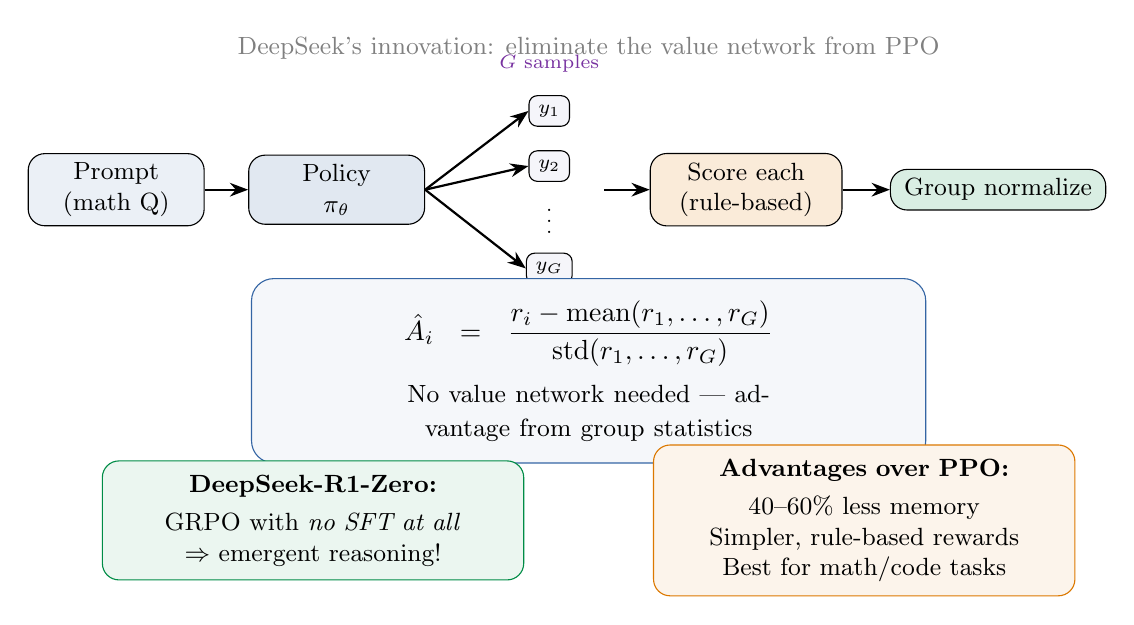
\begin{tikzpicture}
  % Title
  \node[font=\small, text=gray] at (0, 3.3) {DeepSeek's innovation: eliminate the value network from PPO};

  % Process
  \node[draw, rounded corners=6pt, fill=popblue!10, font=\small, text width=2cm, align=center] (prompt) at (-6, 1.5) {Prompt\\(math Q)};
  \node[draw, rounded corners=6pt, fill=popblue!15, font=\small, text width=2cm, align=center] (policy) at (-3.2, 1.5) {Policy\\$\pi_\theta$};

  % G responses
  \node[draw, rounded corners=3pt, fill=lightbg, font=\scriptsize] (r1) at (-0.5, 2.5) {$y_1$};
  \node[draw, rounded corners=3pt, fill=lightbg, font=\scriptsize] (r2) at (-0.5, 1.8) {$y_2$};
  \node[font=\scriptsize] at (-0.5, 1.2) {$\vdots$};
  \node[draw, rounded corners=3pt, fill=lightbg, font=\scriptsize] (rg) at (-0.5, 0.5) {$y_G$};

  \draw[-Stealth, thick] (prompt) -- (policy);
  \draw[-Stealth, thick] (policy.east) -- (r1.west);
  \draw[-Stealth, thick] (policy.east) -- (r2.west);
  \draw[-Stealth, thick] (policy.east) -- (rg.west);

  \node[font=\scriptsize, text=violet1] at (-0.5, 3.1) {$G$ samples};

  % Score
  \node[draw, rounded corners=6pt, fill=orange1!15, font=\small, text width=2.2cm, align=center] (score) at (2, 1.5) {Score each\\(rule-based)};
  \draw[-Stealth, thick] (0.2, 1.5) -- (score.west);

  % Normalize
  \node[draw, rounded corners=6pt, fill=paramgreen!15, font=\small, text width=2.5cm, align=center] (norm) at (5.2, 1.5) {Group normalize};
  \draw[-Stealth, thick] (score) -- (norm);

  % Formula
  \node[draw=popblue, fill=popblue!5, rounded corners=8pt, inner sep=8pt, text width=8cm, align=center] at (0, -0.8) {
    {\normalsize $\displaystyle \hat{A}_i = \frac{r_i - \text{mean}(r_1, \ldots, r_G)}{\text{std}(r_1, \ldots, r_G)}$}\\[6pt]
    {\small No value network needed --- advantage from group statistics}
  };

  % Key results
  \node[draw=paramgreen, fill=paramgreen!8, rounded corners=6pt, text width=5cm, align=center, inner sep=5pt, font=\small] at (-3.5, -2.7) {
    \textbf{DeepSeek-R1-Zero:}\\[3pt]
    GRPO with \emph{no SFT at all}\\$\Rightarrow$ emergent reasoning!
  };
  \node[draw=orange1, fill=orange1!8, rounded corners=6pt, text width=5cm, align=center, inner sep=5pt, font=\small] at (3.5, -2.7) {
    \textbf{Advantages over PPO:}\\[3pt]
    40--60\% less memory\\Simpler, rule-based rewards\\Best for math/code tasks
  };
\end{tikzpicture}
\end{center}
\end{frame}

% ============================================================
% GRPO OBJECTIVE DETAILS
% ============================================================
\begin{frame}
\frametitle{GRPO --- the objective in detail}

\vspace{-0.5cm}
\begin{center}
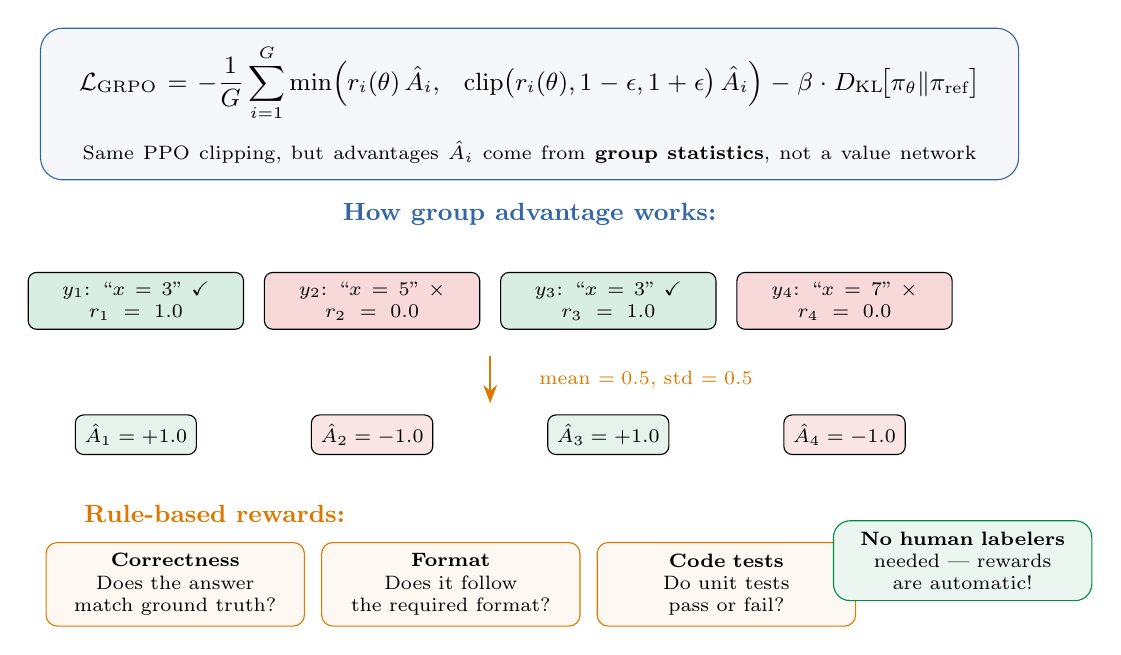
\begin{tikzpicture}
  % Full GRPO objective
  \node[draw=popblue, fill=popblue!5, rounded corners=8pt, inner sep=6pt, text width=12cm, align=center] at (0, 3) {
    {\small $\displaystyle \mathcal{L}_{\text{GRPO}} = -\frac{1}{G}\sum_{i=1}^{G} \min\!\Big(r_i(\theta)\,\hat{A}_i,\;\; \text{clip}\big(r_i(\theta), 1-\epsilon, 1+\epsilon\big)\,\hat{A}_i\Big) - \beta \cdot D_{\text{KL}}\!\big[\pi_\theta \| \pi_{\text{ref}}\big]$}\\[6pt]
    {\scriptsize Same PPO clipping, but advantages $\hat{A}_i$ come from \textbf{group statistics}, not a value network}
  };

  % How it works
  \node[font=\small\bfseries, text=popblue] at (0, 1.6) {How group advantage works:};

  % Visual: G samples with scores
  \node[draw, rounded corners=3pt, fill=paramgreen!15, font=\scriptsize, text width=2.5cm, align=center] at (-5, 0.5) {$y_1$: ``$x=3$'' \checkmark\\$r_1 = 1.0$};
  \node[draw, rounded corners=3pt, fill=sampred!15, font=\scriptsize, text width=2.5cm, align=center] at (-2, 0.5) {$y_2$: ``$x=5$'' $\times$\\$r_2 = 0.0$};
  \node[draw, rounded corners=3pt, fill=paramgreen!15, font=\scriptsize, text width=2.5cm, align=center] at (1, 0.5) {$y_3$: ``$x=3$'' \checkmark\\$r_3 = 1.0$};
  \node[draw, rounded corners=3pt, fill=sampred!15, font=\scriptsize, text width=2.5cm, align=center] at (4, 0.5) {$y_4$: ``$x=7$'' $\times$\\$r_4 = 0.0$};

  \draw[-Stealth, thick, orange1] (-0.5, -0.2) -- (-0.5, -0.8);
  \node[font=\scriptsize, text=orange1, anchor=west] at (0, -0.5) {mean $= 0.5$, std $= 0.5$};

  % Normalized advantages
  \node[draw, rounded corners=3pt, fill=paramgreen!10, font=\scriptsize] at (-5, -1.2) {$\hat{A}_1 = +1.0$};
  \node[draw, rounded corners=3pt, fill=sampred!10, font=\scriptsize] at (-2, -1.2) {$\hat{A}_2 = -1.0$};
  \node[draw, rounded corners=3pt, fill=paramgreen!10, font=\scriptsize] at (1, -1.2) {$\hat{A}_3 = +1.0$};
  \node[draw, rounded corners=3pt, fill=sampred!10, font=\scriptsize] at (4, -1.2) {$\hat{A}_4 = -1.0$};

  % Rule-based rewards
  \node[font=\small\bfseries, text=orange1] at (-4, -2.2) {Rule-based rewards:};

  \node[draw=orange1, fill=orange1!5, rounded corners=4pt, text width=3cm, align=center, inner sep=4pt, font=\scriptsize] at (-4.5, -3.1) {
    \textbf{Correctness}\\Does the answer\\match ground truth?
  };
  \node[draw=orange1, fill=orange1!5, rounded corners=4pt, text width=3cm, align=center, inner sep=4pt, font=\scriptsize] at (-1, -3.1) {
    \textbf{Format}\\Does it follow\\the required format?
  };
  \node[draw=orange1, fill=orange1!5, rounded corners=4pt, text width=3cm, align=center, inner sep=4pt, font=\scriptsize] at (2.5, -3.1) {
    \textbf{Code tests}\\Do unit tests\\pass or fail?
  };

  % Key insight
  \node[draw=paramgreen, fill=paramgreen!8, rounded corners=6pt, text width=3cm, align=center, inner sep=4pt, font=\scriptsize] at (5.5, -2.8) {
    \textbf{No human labelers}\\needed --- rewards\\are automatic!
  };
\end{tikzpicture}
\end{center}
\end{frame}

% ============================================================
% ALIGNMENT COMPARED
% ============================================================
\begin{frame}
\frametitle{Alignment methods compared}

\vspace{-0.1cm}
\renewcommand{\arraystretch}{1.5}
\begin{center}
{\small
\begin{tabular}{>{\bfseries}l c c c c}
  \textbf{Method} & \textbf{Models needed} & \textbf{Stability} & \textbf{Data} & \textbf{Best for} \\
  \hline
  \textcolor{sampred}{RLHF (PPO)} & 4 (policy, ref, RM, value) & Unstable & Preferences & General alignment \\[3pt]
  \textcolor{paramgreen}{DPO} & 2 (policy, ref) & Stable & Preferences & Simple alignment \\[3pt]
  \textcolor{orange1}{GRPO} & 2 (policy, ref) & Medium & Verifiable & Math/code reasoning \\
  \hline
\end{tabular}
}
\end{center}

\vspace{0.4cm}
\begin{center}
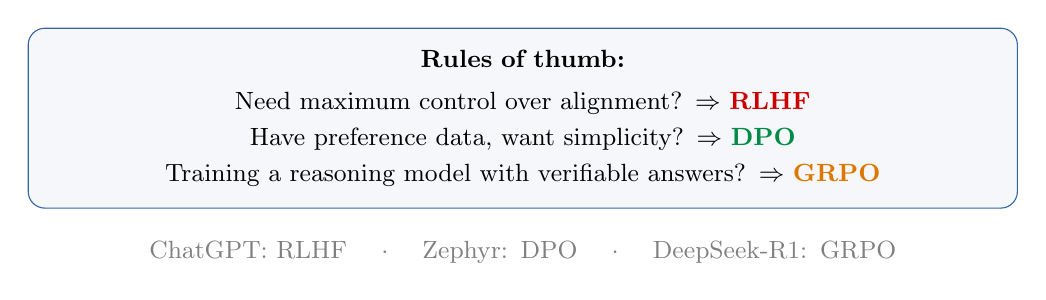
\begin{tikzpicture}
  % Decision guide
  \node[draw=popblue, fill=popblue!5, rounded corners=6pt, text width=12cm, align=center, inner sep=8pt, font=\small] at (0, 0.5) {
    \textbf{Rules of thumb:}\\[4pt]
    Need maximum control over alignment? $\Rightarrow$ \textbf{\textcolor{sampred}{RLHF}}\\[2pt]
    Have preference data, want simplicity? $\Rightarrow$ \textbf{\textcolor{paramgreen}{DPO}}\\[2pt]
    Training a reasoning model with verifiable answers? $\Rightarrow$ \textbf{\textcolor{orange1}{GRPO}}
  };

  % Real examples
  \node[font=\small, text=gray, text width=12cm, align=center] at (0, -1.2) {
    ChatGPT: RLHF \quad $\cdot$ \quad Zephyr: DPO \quad $\cdot$ \quad DeepSeek-R1: GRPO
  };
\end{tikzpicture}
\end{center}
\end{frame}

% ============================================================
% THE COST PROBLEM
% ============================================================
\begin{frame}
\frametitle{The cost problem}

\begin{center}
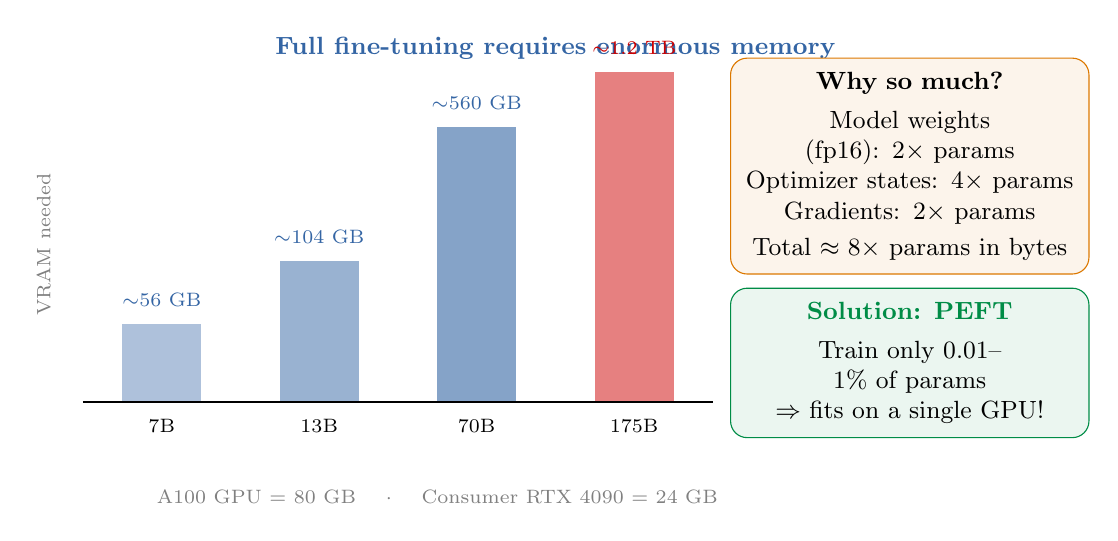
\begin{tikzpicture}
  % Model size → VRAM
  \node[font=\small\bfseries, text=popblue] at (0, 3.5) {Full fine-tuning requires enormous memory};

  % Bar chart (manual)
  % 7B
  \fill[popblue!40] (-5.5, -1) rectangle (-4.5, 0);
  \node[font=\scriptsize] at (-5, -1.3) {7B};
  \node[font=\scriptsize, text=popblue] at (-5, 0.3) {$\sim$56 GB};

  % 13B
  \fill[popblue!50] (-3.5, -1) rectangle (-2.5, 0.8);
  \node[font=\scriptsize] at (-3, -1.3) {13B};
  \node[font=\scriptsize, text=popblue] at (-3, 1.1) {$\sim$104 GB};

  % 70B
  \fill[popblue!60] (-1.5, -1) rectangle (-0.5, 2.5);
  \node[font=\scriptsize] at (-1, -1.3) {70B};
  \node[font=\scriptsize, text=popblue] at (-1, 2.8) {$\sim$560 GB};

  % 175B
  \fill[sampred!50] (0.5, -1) rectangle (1.5, 3.2);
  \node[font=\scriptsize] at (1, -1.3) {175B};
  \node[font=\scriptsize, text=sampred] at (1, 3.5) {$\sim$1.2 TB};

  % Axis
  \draw[thick] (-6, -1) -- (2, -1);
  \node[font=\scriptsize, text=gray, rotate=90] at (-6.5, 1) {VRAM needed};

  % Why 8x
  \node[draw=orange1, fill=orange1!8, rounded corners=6pt, text width=4.2cm, align=center, inner sep=5pt, font=\small] at (4.5, 2) {
    \textbf{Why so much?}\\[3pt]
    Model weights (fp16): $2 \times$ params\\
    Optimizer states: $4 \times$ params\\
    Gradients: $2 \times$ params\\[2pt]
    Total $\approx 8 \times$ params in bytes
  };

  % Solution
  \node[draw=paramgreen, fill=paramgreen!8, rounded corners=6pt, text width=4.2cm, align=center, inner sep=5pt, font=\small] at (4.5, -0.5) {
    \textbf{\textcolor{paramgreen}{Solution: PEFT}}\\[3pt]
    Train only 0.01--1\% of params\\$\Rightarrow$ fits on a single GPU!
  };

  % Consumer GPU reference
  \node[font=\scriptsize, text=gray] at (-1.5, -2.2) {A100 GPU = 80 GB \quad $\cdot$ \quad Consumer RTX 4090 = 24 GB};
\end{tikzpicture}
\end{center}
\end{frame}

% ============================================================
% LoRA
% ============================================================
\begin{frame}
\frametitle{LoRA --- Low-Rank Adaptation}

\vspace{-0.4cm}
\begin{center}
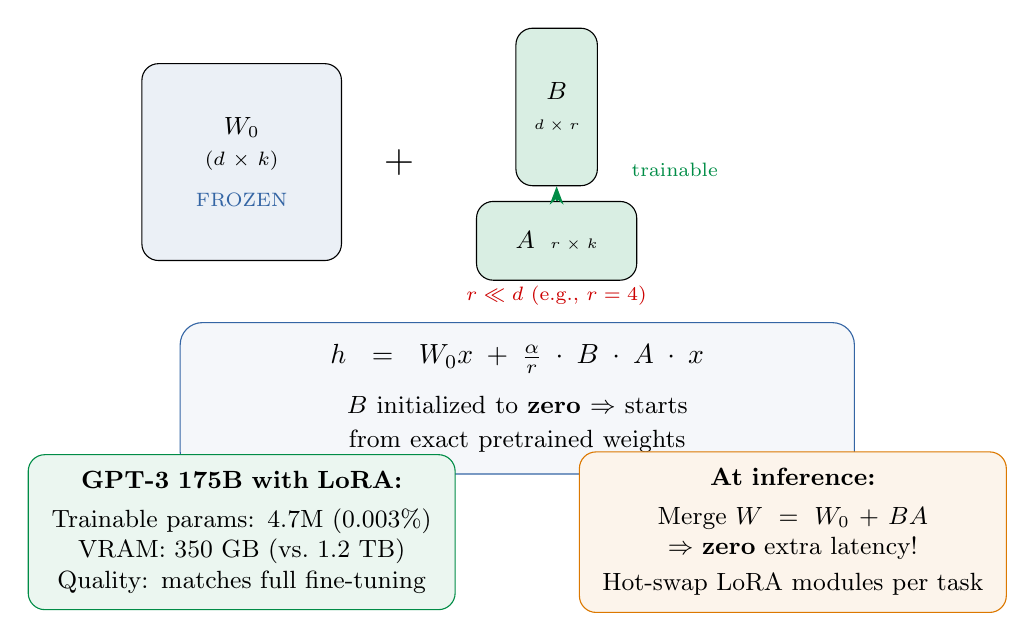
\begin{tikzpicture}
  % Frozen weight
  \node[draw, rounded corners=6pt, fill=popblue!10, minimum width=2.5cm, minimum height=2.5cm, font=\small, text width=2.3cm, align=center] (W) at (-3.5, 1.5) {
    $W_0$\\{\scriptsize $(d \times k)$}\\[4pt]
    {\scriptsize \textcolor{popblue}{FROZEN}}
  };

  % LoRA matrices
  \node[draw, rounded corners=6pt, fill=paramgreen!15, minimum width=1cm, minimum height=2cm, font=\small, text width=0.8cm, align=center] (B) at (0.5, 2.2) {$B$\\{\tiny $d \times r$}};
  \node[draw, rounded corners=6pt, fill=paramgreen!15, minimum width=2cm, minimum height=1cm, font=\small, text width=1.8cm, align=center] (A) at (0.5, 0.5) {$A$ \;{\tiny $r \times k$}};
  \draw[-Stealth, thick, paramgreen] (A) -- (B);
  \node[font=\scriptsize, text=paramgreen] at (2, 1.4) {trainable};
  \node[font=\scriptsize, text=sampred] at (0.5, -0.2) {$r \ll d$ (e.g., $r = 4$)};

  % Plus
  \node[font=\Large] at (-1.5, 1.5) {$+$};

  % Formula
  \node[draw=popblue, fill=popblue!5, rounded corners=8pt, inner sep=8pt, text width=8cm, align=center] at (0, -1.5) {
    {\normalsize $h = W_0 x + \frac{\alpha}{r} \cdot B \cdot A \cdot x$}\\[6pt]
    {\small $B$ initialized to \textbf{zero} $\Rightarrow$ starts from exact pretrained weights}
  };

  % Key results
  \node[draw=paramgreen, fill=paramgreen!8, rounded corners=6pt, text width=5cm, align=center, inner sep=6pt, font=\small] at (-3.5, -3.2) {
    \textbf{GPT-3 175B with LoRA:}\\[3pt]
    Trainable params: 4.7M (0.003\%)\\VRAM: 350 GB (vs.\ 1.2 TB)\\Quality: matches full fine-tuning
  };
  \node[draw=orange1, fill=orange1!8, rounded corners=6pt, text width=5cm, align=center, inner sep=6pt, font=\small] at (3.5, -3.2) {
    \textbf{At inference:}\\[3pt]
    Merge $W = W_0 + BA$\\$\Rightarrow$ \textbf{zero} extra latency!\\[2pt]
    Hot-swap LoRA modules per task
  };
\end{tikzpicture}
\end{center}
\end{frame}

% ============================================================
% PEFT METHODS
% ============================================================
\begin{frame}
\frametitle{PEFT methods compared}

\vspace{-0.1cm}
\renewcommand{\arraystretch}{1.4}
\begin{center}
{\small
\begin{tabular}{>{\bfseries}l l c c c}
  \textbf{Method} & \textbf{Approach} & \textbf{Params} & \textbf{Inference} & \textbf{Quality} \\
  \hline
  \textcolor{paramgreen}{LoRA} & Low-rank update to $W$ & $\sim$0.01\% & No overhead & Excellent \\[2pt]
  \textcolor{popblue}{Adapters} & New layers between blocks & $\sim$1--5\% & +20--30\% & Excellent \\[2pt]
  \textcolor{orange1}{Prefix tuning} & Learnable prefix to $K$, $V$ & $\sim$0.1\% & Slight & Good \\[2pt]
  \textcolor{violet1}{Prompt tuning} & Soft prompt embeddings & $\sim$0.01\% & Slight & Good \\[2pt]
  \textcolor{sampred}{Full FT} & Update all weights & 100\% & Baseline & Best \\
  \hline
\end{tabular}
}
\end{center}

\vspace{0.3cm}
\begin{center}
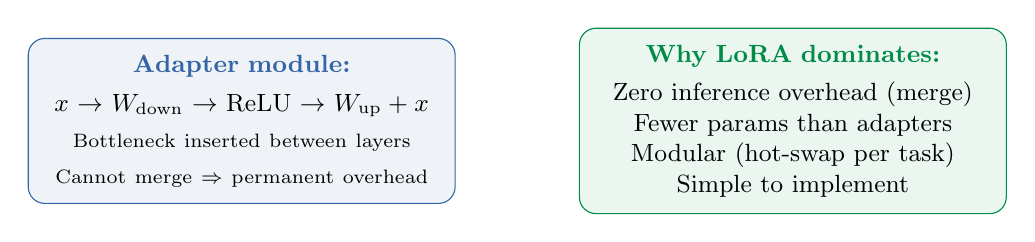
\begin{tikzpicture}
  % Adapter diagram (compact)
  \node[draw=popblue, fill=popblue!8, rounded corners=6pt, text width=5cm, align=center, inner sep=6pt, font=\small] at (-3.5, 0) {
    \textbf{\textcolor{popblue}{Adapter module:}}\\[3pt]
    $x \to W_{\text{down}} \to \text{ReLU} \to W_{\text{up}} + x$\\[2pt]
    {\scriptsize Bottleneck inserted between layers}\\[2pt]
    {\scriptsize Cannot merge $\Rightarrow$ permanent overhead}
  };

  % LoRA advantage
  \node[draw=paramgreen, fill=paramgreen!8, rounded corners=6pt, text width=5cm, align=center, inner sep=6pt, font=\small] at (3.5, 0) {
    \textbf{\textcolor{paramgreen}{Why LoRA dominates:}}\\[3pt]
    Zero inference overhead (merge)\\Fewer params than adapters\\Modular (hot-swap per task)\\Simple to implement
  };
\end{tikzpicture}
\end{center}
\end{frame}

% ============================================================
% THE FULL PICTURE
% ============================================================
\begin{frame}
\frametitle{The full picture}

\begin{center}
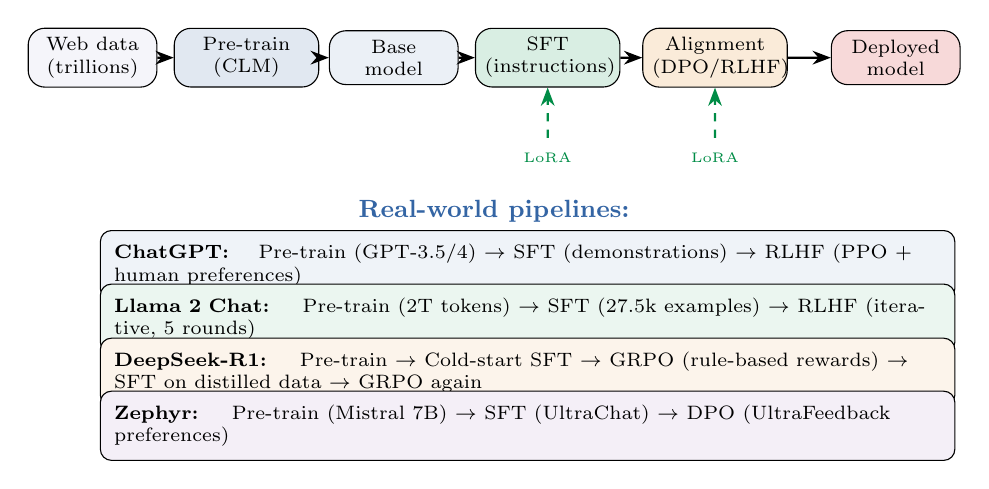
\begin{tikzpicture}[scale=0.85]
  % Pipeline
  \node[draw, rounded corners=6pt, fill=lightbg, font=\scriptsize, text width=1.4cm, align=center] (data) at (-6.5, 2) {Web data\\(trillions)};
  \node[draw, rounded corners=6pt, fill=popblue!15, font=\scriptsize, text width=1.6cm, align=center] (pt) at (-4.2, 2) {Pre-train\\(CLM)};
  \node[draw, rounded corners=6pt, fill=popblue!10, font=\scriptsize, text width=1.4cm, align=center] (base) at (-2, 2) {Base\\model};
  \node[draw, rounded corners=6pt, fill=paramgreen!15, font=\scriptsize, text width=1.6cm, align=center] (sft) at (0.3, 2) {SFT\\(instructions)};
  \node[draw, rounded corners=6pt, fill=orange1!15, font=\scriptsize, text width=1.6cm, align=center] (align) at (2.8, 2) {Alignment\\(DPO/RLHF)};
  \node[draw, rounded corners=6pt, fill=sampred!15, font=\scriptsize, text width=1.4cm, align=center] (dep) at (5.5, 2) {Deployed\\model};

  \draw[-Stealth, thick] (data) -- (pt);
  \draw[-Stealth, thick] (pt) -- (base);
  \draw[-Stealth, thick] (base) -- (sft);
  \draw[-Stealth, thick] (sft) -- (align);
  \draw[-Stealth, thick] (align) -- (dep);

  % LoRA annotations
  \draw[-Stealth, thick, paramgreen, dashed] (0.3, 0.8) -- (sft.south);
  \node[font=\tiny, text=paramgreen] at (0.3, 0.5) {LoRA};
  \draw[-Stealth, thick, paramgreen, dashed] (2.8, 0.8) -- (align.south);
  \node[font=\tiny, text=paramgreen] at (2.8, 0.5) {LoRA};

  % Real examples
  \node[font=\small\bfseries, text=popblue] at (-0.5, -0.3) {Real-world pipelines:};

  % ChatGPT
  \node[draw, rounded corners=4pt, fill=popblue!8, text width=10.5cm, align=left, inner sep=5pt, font=\scriptsize] at (0, -1.1) {
    \textbf{ChatGPT:} \quad Pre-train (GPT-3.5/4) $\to$ SFT (demonstrations) $\to$ RLHF (PPO + human preferences)
  };
  % Llama
  \node[draw, rounded corners=4pt, fill=paramgreen!8, text width=10.5cm, align=left, inner sep=5pt, font=\scriptsize] at (0, -1.9) {
    \textbf{Llama 2 Chat:} \quad Pre-train (2T tokens) $\to$ SFT (27.5k examples) $\to$ RLHF (iterative, 5 rounds)
  };
  % DeepSeek
  \node[draw, rounded corners=4pt, fill=orange1!8, text width=10.5cm, align=left, inner sep=5pt, font=\scriptsize] at (0, -2.7) {
    \textbf{DeepSeek-R1:} \quad Pre-train $\to$ Cold-start SFT $\to$ GRPO (rule-based rewards) $\to$ SFT on distilled data $\to$ GRPO again
  };
  % Zephyr
  \node[draw, rounded corners=4pt, fill=violet1!8, text width=10.5cm, align=left, inner sep=5pt, font=\scriptsize] at (0, -3.5) {
    \textbf{Zephyr:} \quad Pre-train (Mistral 7B) $\to$ SFT (UltraChat) $\to$ DPO (UltraFeedback preferences)
  };
\end{tikzpicture}
\end{center}
\end{frame}

% ============================================================
% PRACTICAL GUIDE
% ============================================================
\begin{frame}
\frametitle{Practical guide}

\vspace{-0.2cm}
\begin{center}
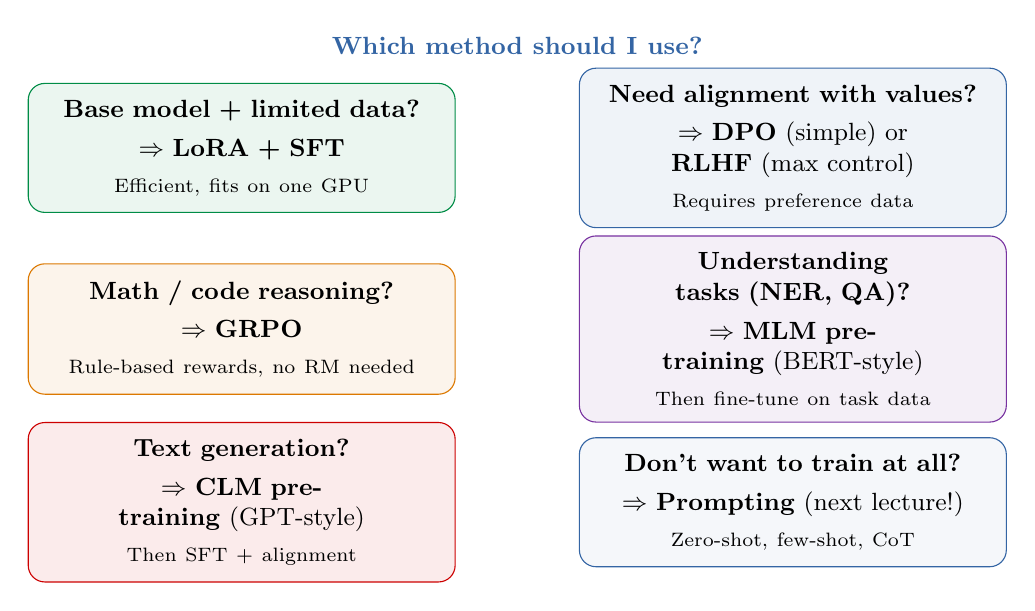
\begin{tikzpicture}
  \node[font=\small\bfseries, text=popblue] at (0, 3.3) {Which method should I use?};

  % Decision boxes
  \node[draw=paramgreen, fill=paramgreen!8, rounded corners=6pt, text width=5cm, align=center, inner sep=6pt, font=\small] at (-3.5, 2) {
    \textbf{Base model + limited data?}\\[3pt]
    $\Rightarrow$ \textbf{LoRA + SFT}\\[2pt]
    {\scriptsize Efficient, fits on one GPU}
  };
  \node[draw=popblue, fill=popblue!8, rounded corners=6pt, text width=5cm, align=center, inner sep=6pt, font=\small] at (3.5, 2) {
    \textbf{Need alignment with values?}\\[3pt]
    $\Rightarrow$ \textbf{DPO} (simple) or \textbf{RLHF} (max control)\\[2pt]
    {\scriptsize Requires preference data}
  };
  \node[draw=orange1, fill=orange1!8, rounded corners=6pt, text width=5cm, align=center, inner sep=6pt, font=\small] at (-3.5, -0.3) {
    \textbf{Math / code reasoning?}\\[3pt]
    $\Rightarrow$ \textbf{GRPO}\\[2pt]
    {\scriptsize Rule-based rewards, no RM needed}
  };
  \node[draw=violet1, fill=violet1!8, rounded corners=6pt, text width=5cm, align=center, inner sep=6pt, font=\small] at (3.5, -0.3) {
    \textbf{Understanding tasks (NER, QA)?}\\[3pt]
    $\Rightarrow$ \textbf{MLM pre-training} (BERT-style)\\[2pt]
    {\scriptsize Then fine-tune on task data}
  };
  \node[draw=sampred, fill=sampred!8, rounded corners=6pt, text width=5cm, align=center, inner sep=6pt, font=\small] at (-3.5, -2.5) {
    \textbf{Text generation?}\\[3pt]
    $\Rightarrow$ \textbf{CLM pre-training} (GPT-style)\\[2pt]
    {\scriptsize Then SFT + alignment}
  };
  \node[draw=popblue, fill=popblue!5, rounded corners=6pt, text width=5cm, align=center, inner sep=6pt, font=\small] at (3.5, -2.5) {
    \textbf{Don't want to train at all?}\\[3pt]
    $\Rightarrow$ \textbf{Prompting} (next lecture!)\\[2pt]
    {\scriptsize Zero-shot, few-shot, CoT}
  };
\end{tikzpicture}
\end{center}
\end{frame}

% ============================================================
% QUESTIONS
% ============================================================
\begin{frame}
\begin{center}
\vspace{2cm}
{\Huge \textcolor{popblue}{Questions?}}

\vspace{1cm}
{\large Next: Prompting --- Zero-shot, Few-shot, Chain-of-Thought}
\end{center}
\end{frame}

\end{document}
